\documentclass[t,english]{sdqbeamer}
%\documentclass[c]{sdqbeamer}

\usepackage{listings}
\usepackage{graphicx}
\usepackage{tabularx}
\usepackage{tikzsymbols}
\usepackage{booktabs}

\usepackage[lined,linesnumbered,ruled,noend]{algorithm2e}
\renewcommand{\thealgocf}{}

\hypersetup{
	colorlinks=true,
	urlcolor=kit-green,
	citecolor=mygray
}

% set sdqbeamer options
\titleimage{blender-render}
\groupname{} % rendered at the bottom center of each slide
\grouplogo{ae+satres}
\selectlanguage{english}

% define title etc.pp.
\title{Practical SAT Solving}
\subtitle{Lecture 8 \unimp{\normalfont -- Parallel SAT Solving}}
\author{{Ashlin Iser}, \underline{Dominik Schreiber}}
\date{June 16, 2025}

% define commands
\input{l00-commands.tex}

%\usepackage[english]{babel}
\usepackage[citestyle=numeric,bibstyle=numeric,hyperref,backend=biber,language=auto]{biblatex}
\addbibresource{references.bib}
\bibhang1em
\setbeamertemplate{navigation symbols}{}

\setlength{\itemsep}{1em}

\newcommand{\iflecture}[1]{#1}
\newcommand{\ifresearchtalk}[1]{#1}

\begin{document}

\begin{frame}[title white horizontal, picture=logos/blender-render, kitlogo=rgb]
	\titlepage
\end{frame}

\begin{frame}{Overview}
	\begin{block}{Recap Lecture 7}
		\begin{itemize}
			\item Propagation-based Redundancy notions
			\item Proof systems: Resolution, Extended Resolution, Blocked Clauses, Implication-based Redundancy
			\item Autarkies, Conditional Autarkies, and Satisfaction Driven Clause Learning (SDCL)
		\end{itemize}
	\end{block}
	\begin{blueblock}{Today: Parallel SAT Solving}
		\textbf{Parallel SAT solving approaches}
		\begin{itemize}
			\item Basic search space splitting, Clause sharing, Cube\&Conquer, Portfolio solvers
		\end{itemize}
		\vspace{0.2cm}
		\textbf{A deep dive into Mallob}
		\begin{itemize}
			\item Overview, Scalable clause sharing, Experiments and insights
		\end{itemize}
	\end{blueblock}
	
\end{frame}

\begin{frame}{Parallel Solving: An analogy}
	\begin{minipage}{0.5\textwidth}
		\begin{blueblock}{The Assembly of Nerds~\cite{schreiber2024mallobsat}}
			\begin{itemize}
				\item Complex and large \highl{logic puzzle}
				\item \highl{$n$ puzzle experts} at your disposition\\
				--- \highlo{anti-social}: work best if left undisturbed				
			\end{itemize}
		\end{blueblock}
		\vspace*{0.3cm}
		\textbf{How do we employ and ``orchestrate'' our experts?}
	\end{minipage}%
	\begin{minipage}{0.5\textwidth}
		\centering
		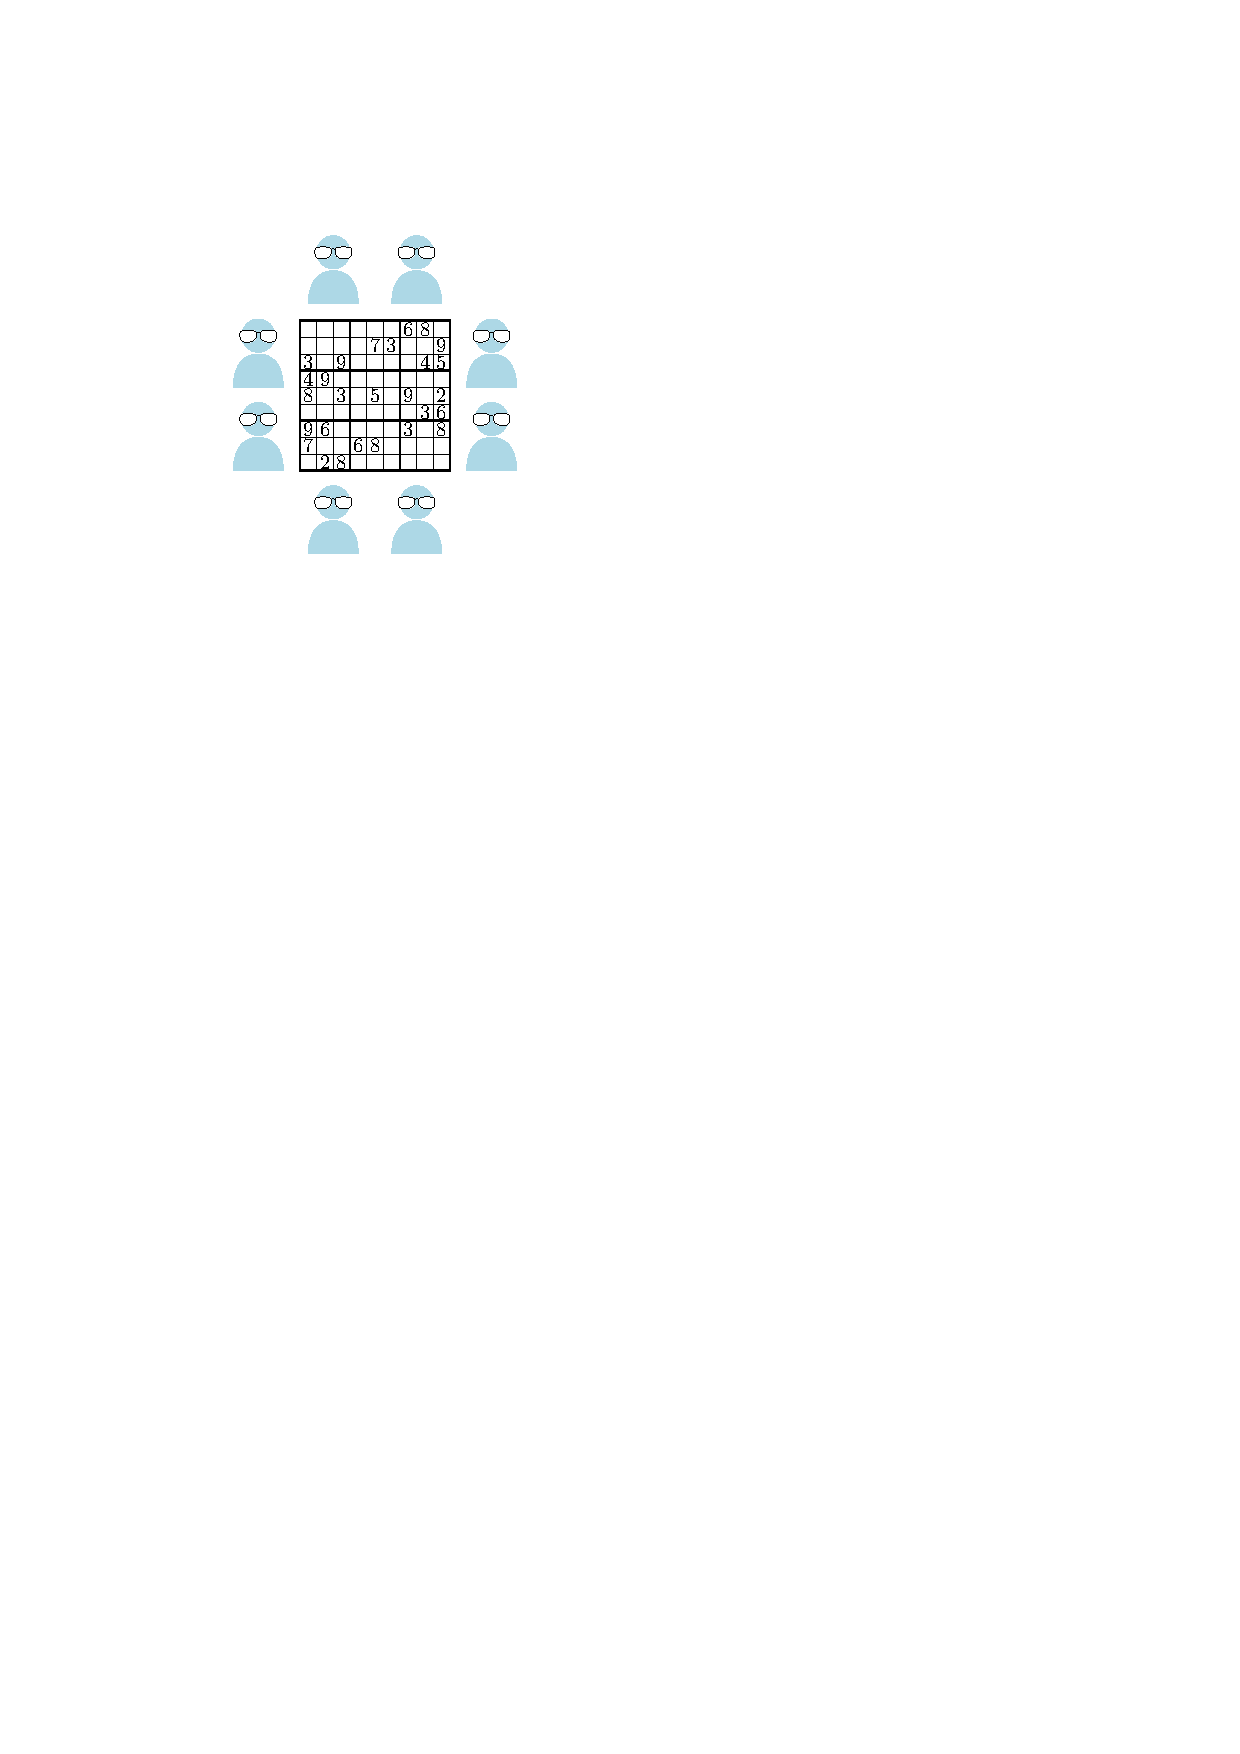
\includegraphics[width=10.8cm]{figures/l08/sudoku-1.pdf}	
	\end{minipage}
\end{frame}

\begin{frame}{Approach I: Search Space Partitioning}
	\begin{minipage}{0.6\textwidth}
		\vspace{0.2cm}
		\hspace*{-0.4cm}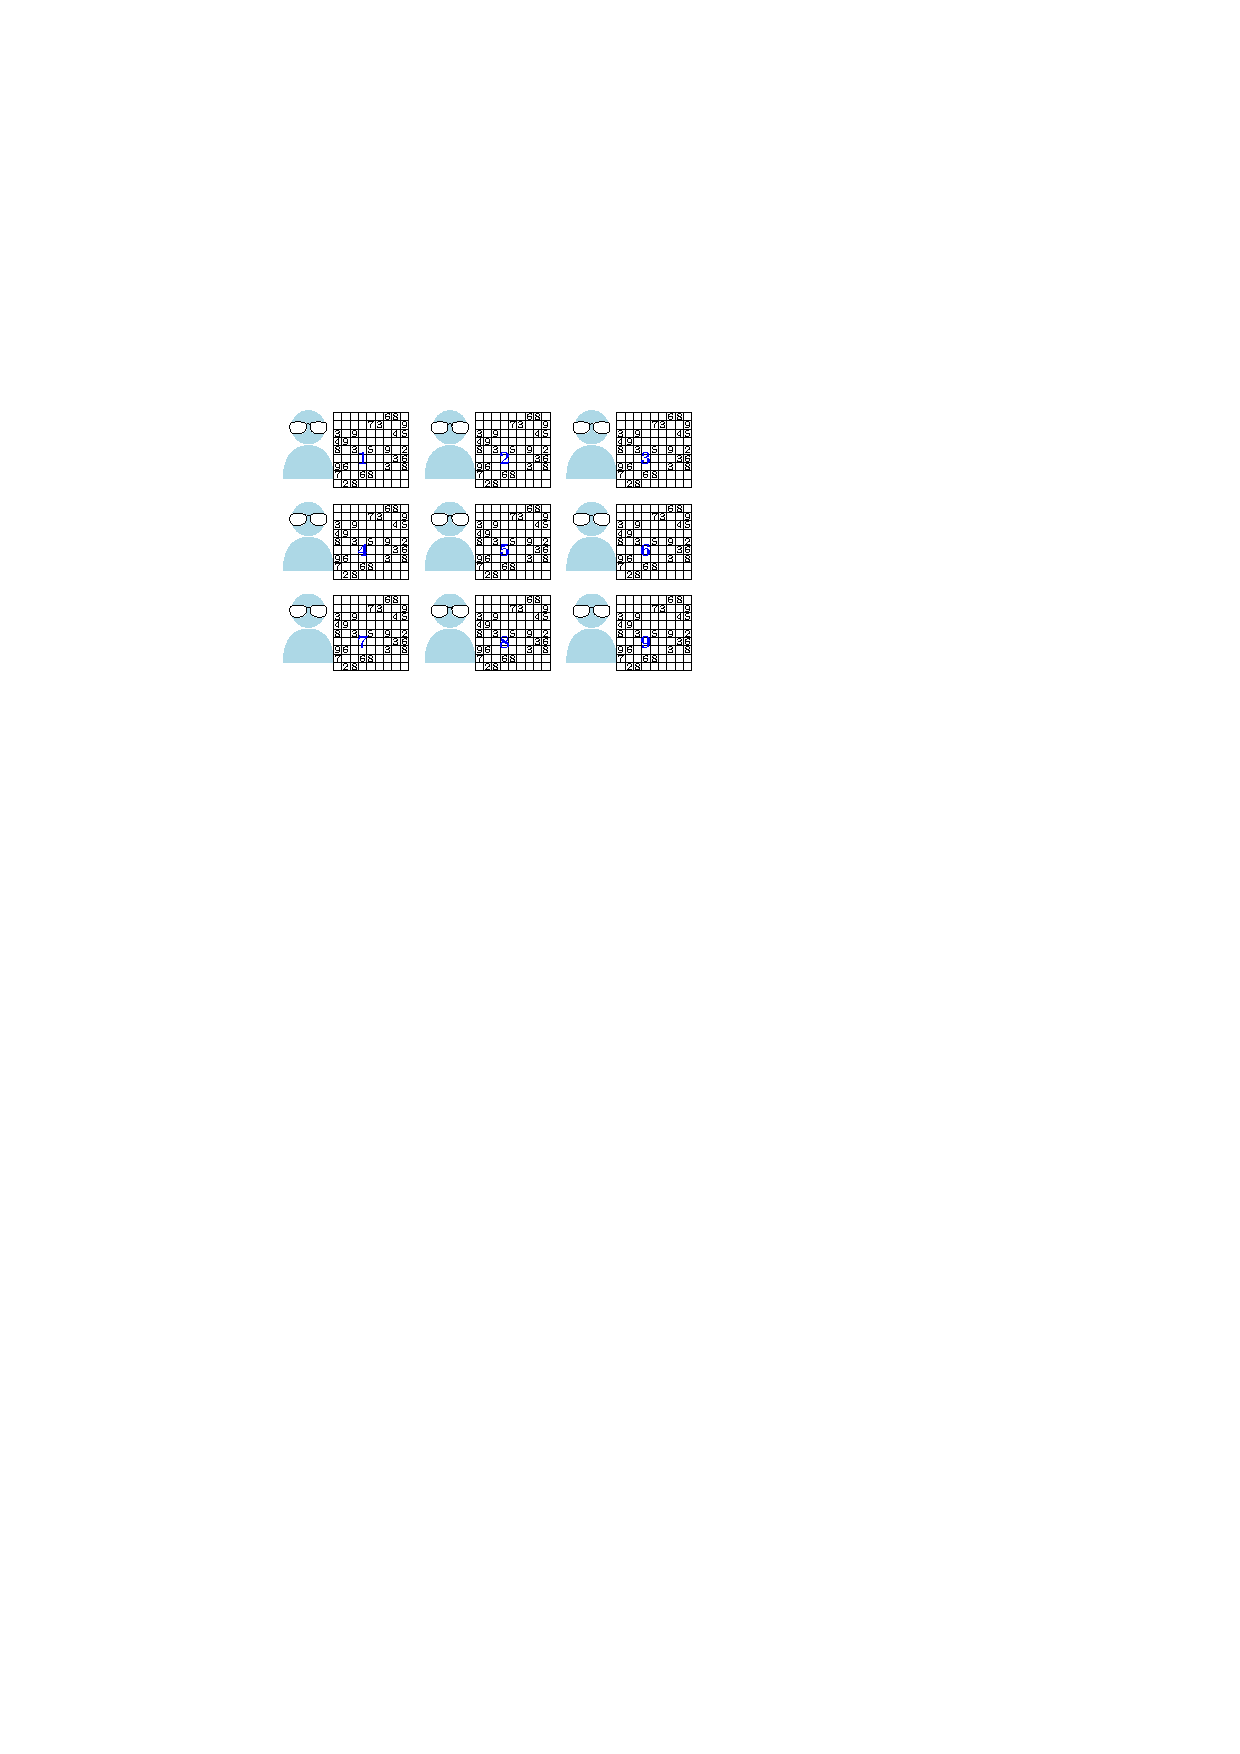
\includegraphics[width=\textwidth]{figures/l08/sudoku-searchspacesplitting.pdf}
	\end{minipage}\quad%
	\begin{minipage}{0.38\textwidth}
		\begin{itemize}
			\pause
			\item \highl{Partition search space} at some decisions\\
			$\Rightarrow$ \highl{Independent subproblems}
			%\item Difficult to \highlo{balance the load}\\
			%--- \highlo{uneven splits}\\
			%--- splits which \highlo{multiply the work}!
			%\pause
			%\vspace{0.5cm}
			%\item \highl{Cube\&Conquer}: Generate many (e.g., millions) of subproblems, \highl{distribute evenly}
			%\item Often relies on \highlo{hand-crafted splitting} for good performance
			%\item Great for theorem proving
			%\item Not today's topic
		\end{itemize}
	\end{minipage}
\end{frame}

\begin{frame}{Explicit Partitioning}
	
	\textbf{Böhm \& Speckenmeyer (1994-1996)}~\cite{bohm1996fast}: 1st Parallel DPLL Implementation\\[3mm]
	
	\begin{blueblock}{Explicit Load Balancing}
		\begin{itemize}
			\item Completely distributed (no leader / worker roles)
			\item A list of \highl{partial assignments} is generated
			\item Each process receives the entire formula and \highl{a few partial assignments}
			\item Each process can be worker or balancer:
			\begin{itemize}
				\item \highl{Worker}: solve or split the formula, use the partial assignments
				\item \highl{Balancer}: estimate workload, communicate, stop
			\end{itemize}
			\item Switch to balancer whenever worker is finished
		\end{itemize}
	\end{blueblock}
\end{frame}

\begin{frame}{Explicit Partitioning}
	
	``\textbf{PSATO}: a Distributed Propositional Prover and its Application to Quasigroup Problems'', Zhang et al. (1996)~\cite{zhang1996psato}\\[3mm]
	
	\begin{blueblock}{Centralized leader-worker architecture}
		\begin{itemize}
			\item Communication only between leader and workers
			\item Leader assigns partial assignments using \highl{Guiding Path}
			\begin{itemize}
				\item Each node in the search tree is \highl{open or closed}\\
				--- closed = branch is \highlo{explored / proven unsat}
				\item Leader splits open nodes and assigns job to workers
			\end{itemize}
			%\item All processors can get stuck on unpromising branches
			\item Workers return \highl{Guiding Path} when terminated by leader
			\item Modern features of \highl{fault tolerance}, \highl{preemption} of solving tasks
		\end{itemize}
	\end{blueblock}
\end{frame}


\begin{frame}{Explicit Partitioning}
	\vspace*{-5mm}
	\textbf{Guiding Path}: \highl{List of triples} (variable, branch, open)
	
	\vspace*{0.3cm}
	\centering
	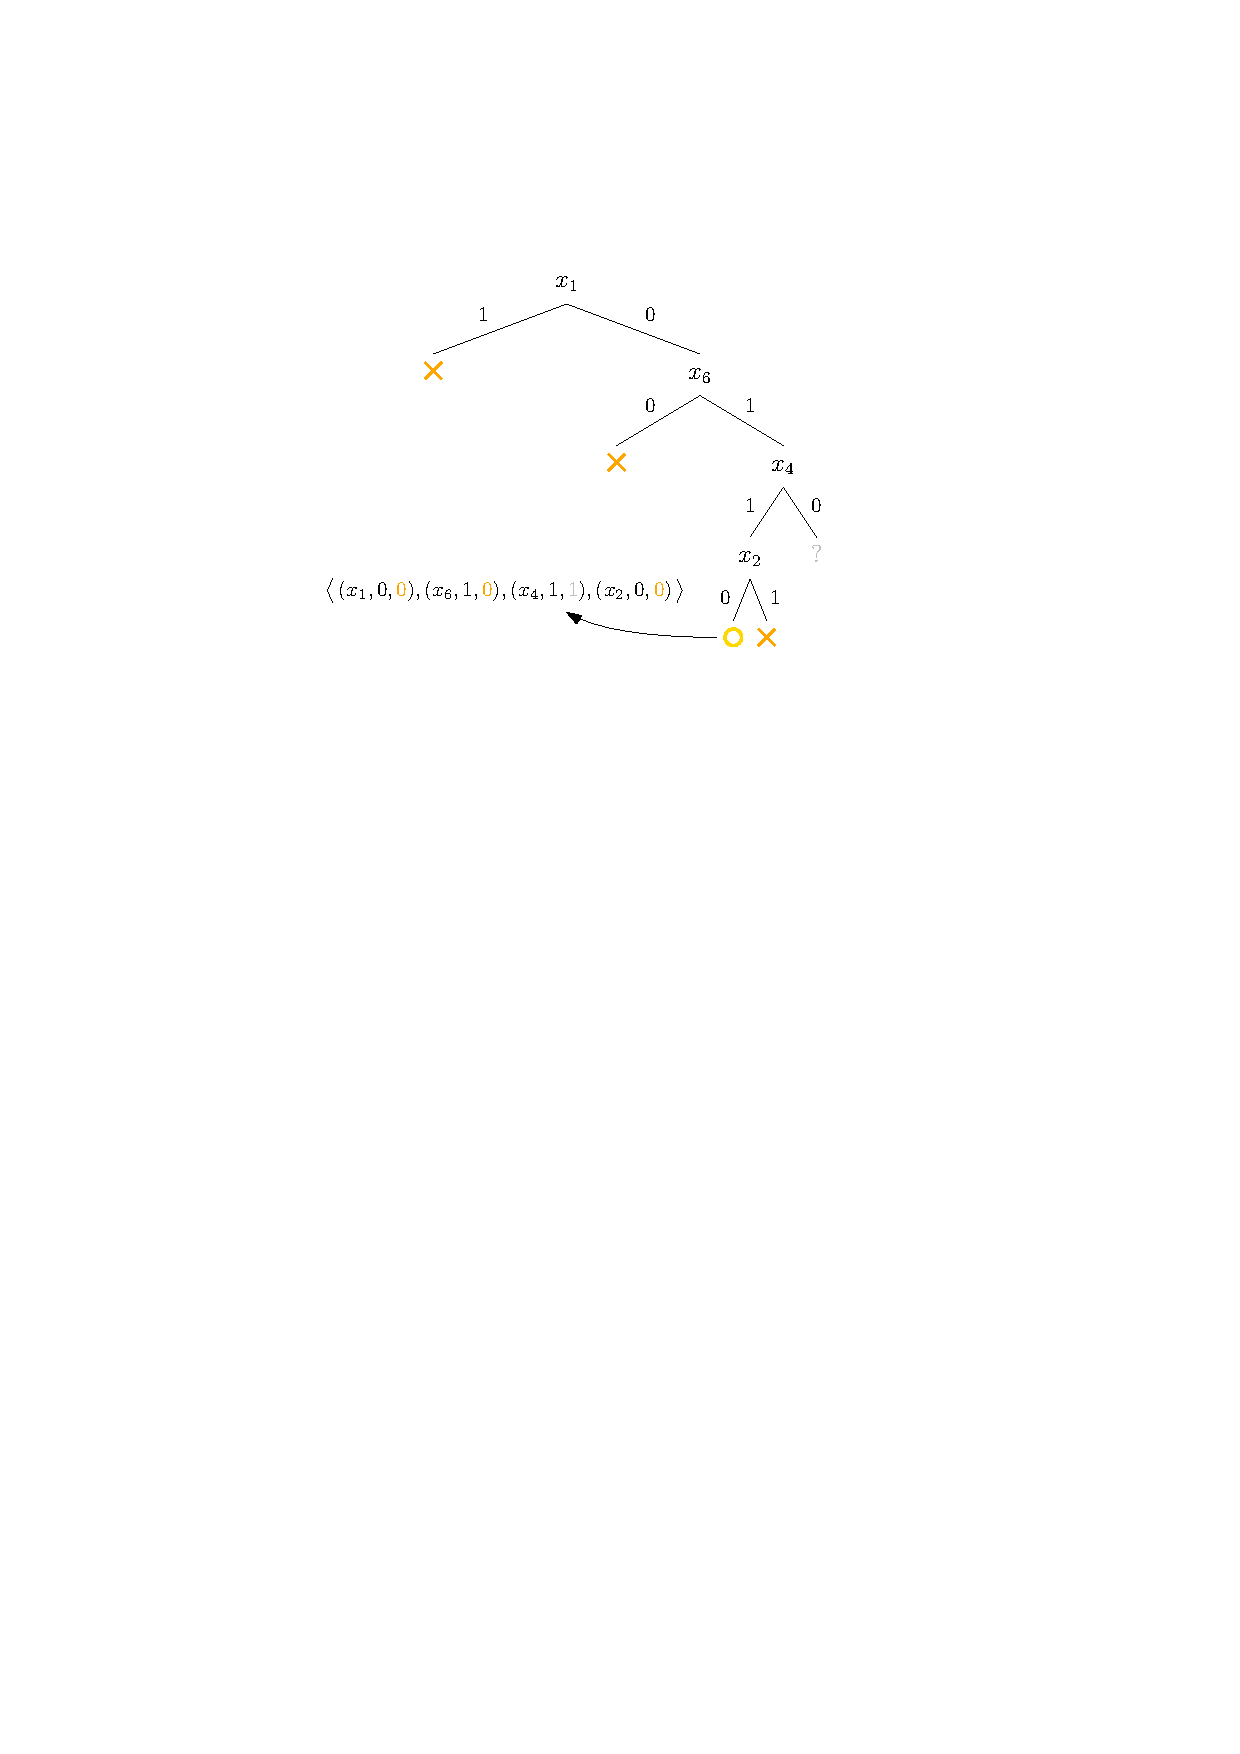
\includegraphics[width=0.5\textwidth]{figures/l08/guiding-path.pdf}
\end{frame}


\begin{frame}{Explicit Partitioning Solvers}
	
	\begin{blueblock}{{SATZ} (Jurkowiak et al., 2001)~\cite{jurkowiak2001parallelizing}: \emph{Work stealing} for workload balancing}
		\begin{itemize}
			\item An idle worker \highl{requests work} from the leader
			\item The leader \highl{splits the work} of the most loaded worker
			\item The idle worker and most loaded worker get the parts
		\end{itemize}
	\end{blueblock}
	\begin{blueblock}{PaSAT (Blochinger et al., 2001-2003)~\cite{blochinger2003parallel}} 
		\begin{itemize}
			\item First parallel CDCL with \highl{clause sharing}
			\item Similar to PSATO/SATZ: leader/worker, guiding path, work stealing
		\end{itemize}
	\end{blueblock}
	\begin{blueblock}{ySAT (Feldman et al., 2004)~\cite{feldman2005parallel}}
		\begin{itemize}
			\item First \highl{shared-memory parallel} solver
			\item Multi-core processors started to be popular
			\item uses same techniques as the previous solvers (guiding path etc.)
			%\item bad performance explained by high number of cache misses (DPLL/CDCL is otherwise highly optimized for cache)
		\end{itemize}
	\end{blueblock}\textbf{}
\end{frame}


%\begin{frame}{1996 -- Clause learning invented}
%	\begin{center}
	%		
\includegraphics[scale=0.5]{figures/l08/learning-meme.jpg}
	%	\end{center}
%\end{frame}

\begin{frame}{Problems with Partitioning~\cite{schulz2010cooperate}}
	\begin{minipage}{0.4\textwidth}
		\centering
		\only<1>{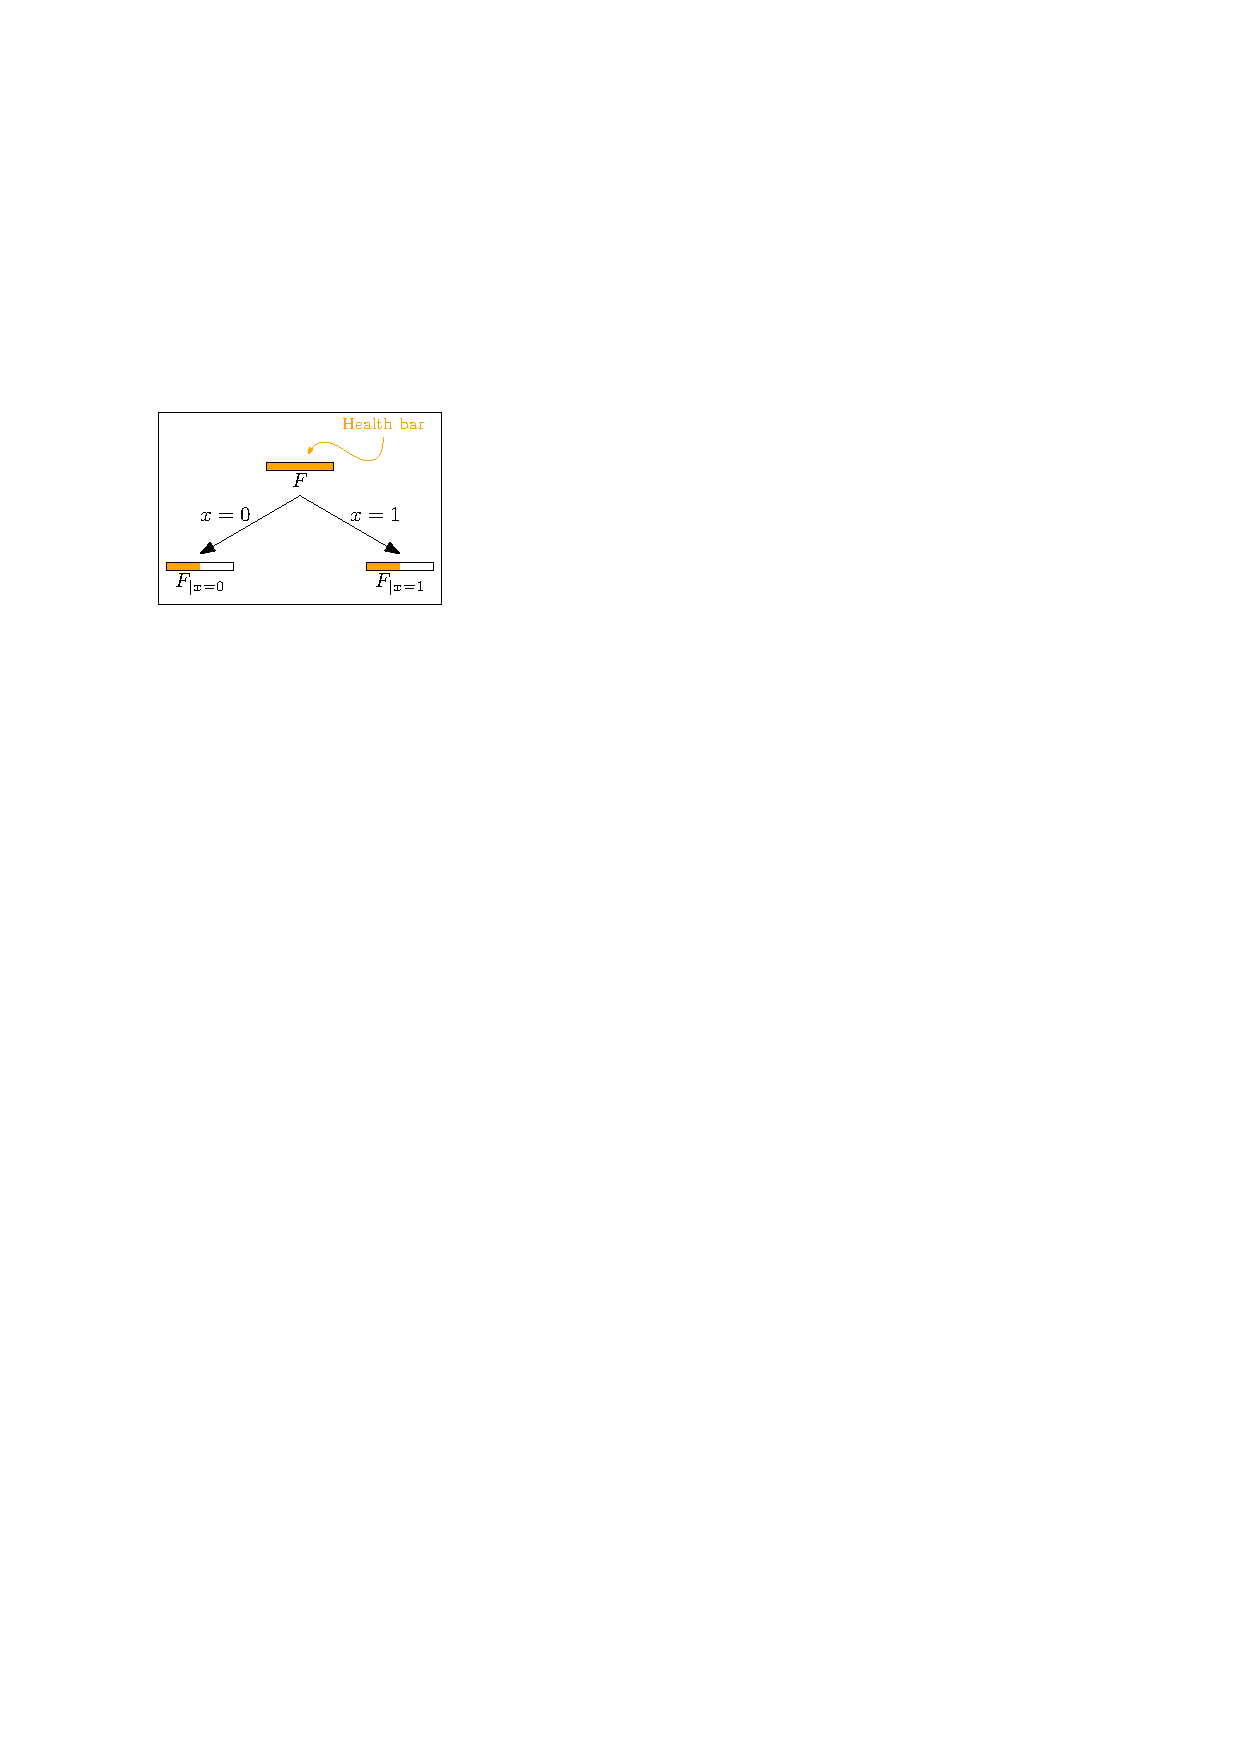
\includegraphics[width=0.8\textwidth,trim=1mm 1mm 1mm 1mm,clip,page=1]{figures/l08/formula-split.pdf}}%
		\only<2>{\includegraphics[width=0.8\textwidth,trim=1mm 1mm 1mm 1mm,clip,page=2]{figures/l08/formula-split.pdf}}%
		\only<3>{\includegraphics[width=0.8\textwidth,trim=1mm 1mm 1mm 1mm,clip,page=3]{figures/l08/formula-split.pdf}}%
	\end{minipage}\quad\quad%
	\begin{minipage}{0.56\textwidth}
		\vspace*{6mm}
		What we want: \textbf{Even splits}
		\begin{itemize}
			\item Split yields sub-formulas of \highl{similar difficulty}
			\item Balanced partitioning of work
			\item Few or no dynamic (re-)balancing needed
		\end{itemize}
		\pause
		\vspace*{0.2cm}
		\textbf{Uneven splits}
		\begin{itemize}
			\item One subformula is \highl{trivial}, the other is \highlo{just as hard as $F$}
			\item \highlo{Ping-pong effect} for workers processing trivial formulae,
			communication / synchronization dominates run time
		\end{itemize}
		\pause
		\vspace*{0.2cm}
		\textbf{Bogus splits}
		\begin{itemize}
			\item Both $F_{|x=0}$ and $F_{|x=1}$ are \highlo{just as hard as $F$}
			\item \highl{Divide\&Conquer} becomes \highlo{Multiply\&Surrender}!
		\end{itemize}
	\end{minipage}
\end{frame}

\begin{frame}{Cube and Conquer}
	\begin{blueblock}{The Cube\&Conquer paradigm (Heule \& Biere, 2011)~\cite{heule2011cube}}
		Generate a large amount (\highl{millions}) of \highl{partial assignments} (``\textbf{cubes}'')
		and \highl{randomly assign} them to workers.		
	\end{blueblock}
	\pause
	\begin{itemize}
		\item Unlikely that any of the workers will run out tasks\\
		$\Rightarrow$ Hope of \highl{good load balancing} in practice
		\item Partial assignments are generated using a \highl{look-ahead solver}\\
		(breadth-first search up to a limited depth)
		\item Best performance mostly with \highlo{problem-specific decision heuristics}
		\pause
		\vspace*{1mm}
		\item State-of-the-art for \highl{hard combinatorial problems}
		\begin{itemize}
			\item Used to solve the ``Pythagorean Triples'' problem ($\sim$200TB proof)~\cite{heule2016solving}
			\item ... or more recently ``Schur Number 5'' ($\sim$2PB proof)~\cite{heule2018schur}
		\end{itemize}
		\item Examples: March (Heule) + iLingeling (Biere) introduced in 2011; Treengeling (Biere)~\cite{biere2013lingeling}
	\end{itemize}
\end{frame}

\begin{frame}{Parallel Portfolios: An analogy}
	\begin{minipage}{0.5\textwidth}
		\begin{blueblock}{The Assembly of Nerds}
			\begin{itemize}
				\item Complex and large \highl{logic puzzle}
				\item \highl{$n$ puzzle experts} at your disposition\\
				--- \highl{individual mindsets}, approaches,\\
				\hspace*{0.37cm}strengths \& weaknesses\\
				--- \highlo{anti-social}: work best if left undisturbed				
			\end{itemize}
		\end{blueblock}
		\vspace*{0.3cm}
		\textbf{How do we employ and ``orchestrate'' our experts?}
	\end{minipage}%
	\begin{minipage}{0.5\textwidth}
		\centering
		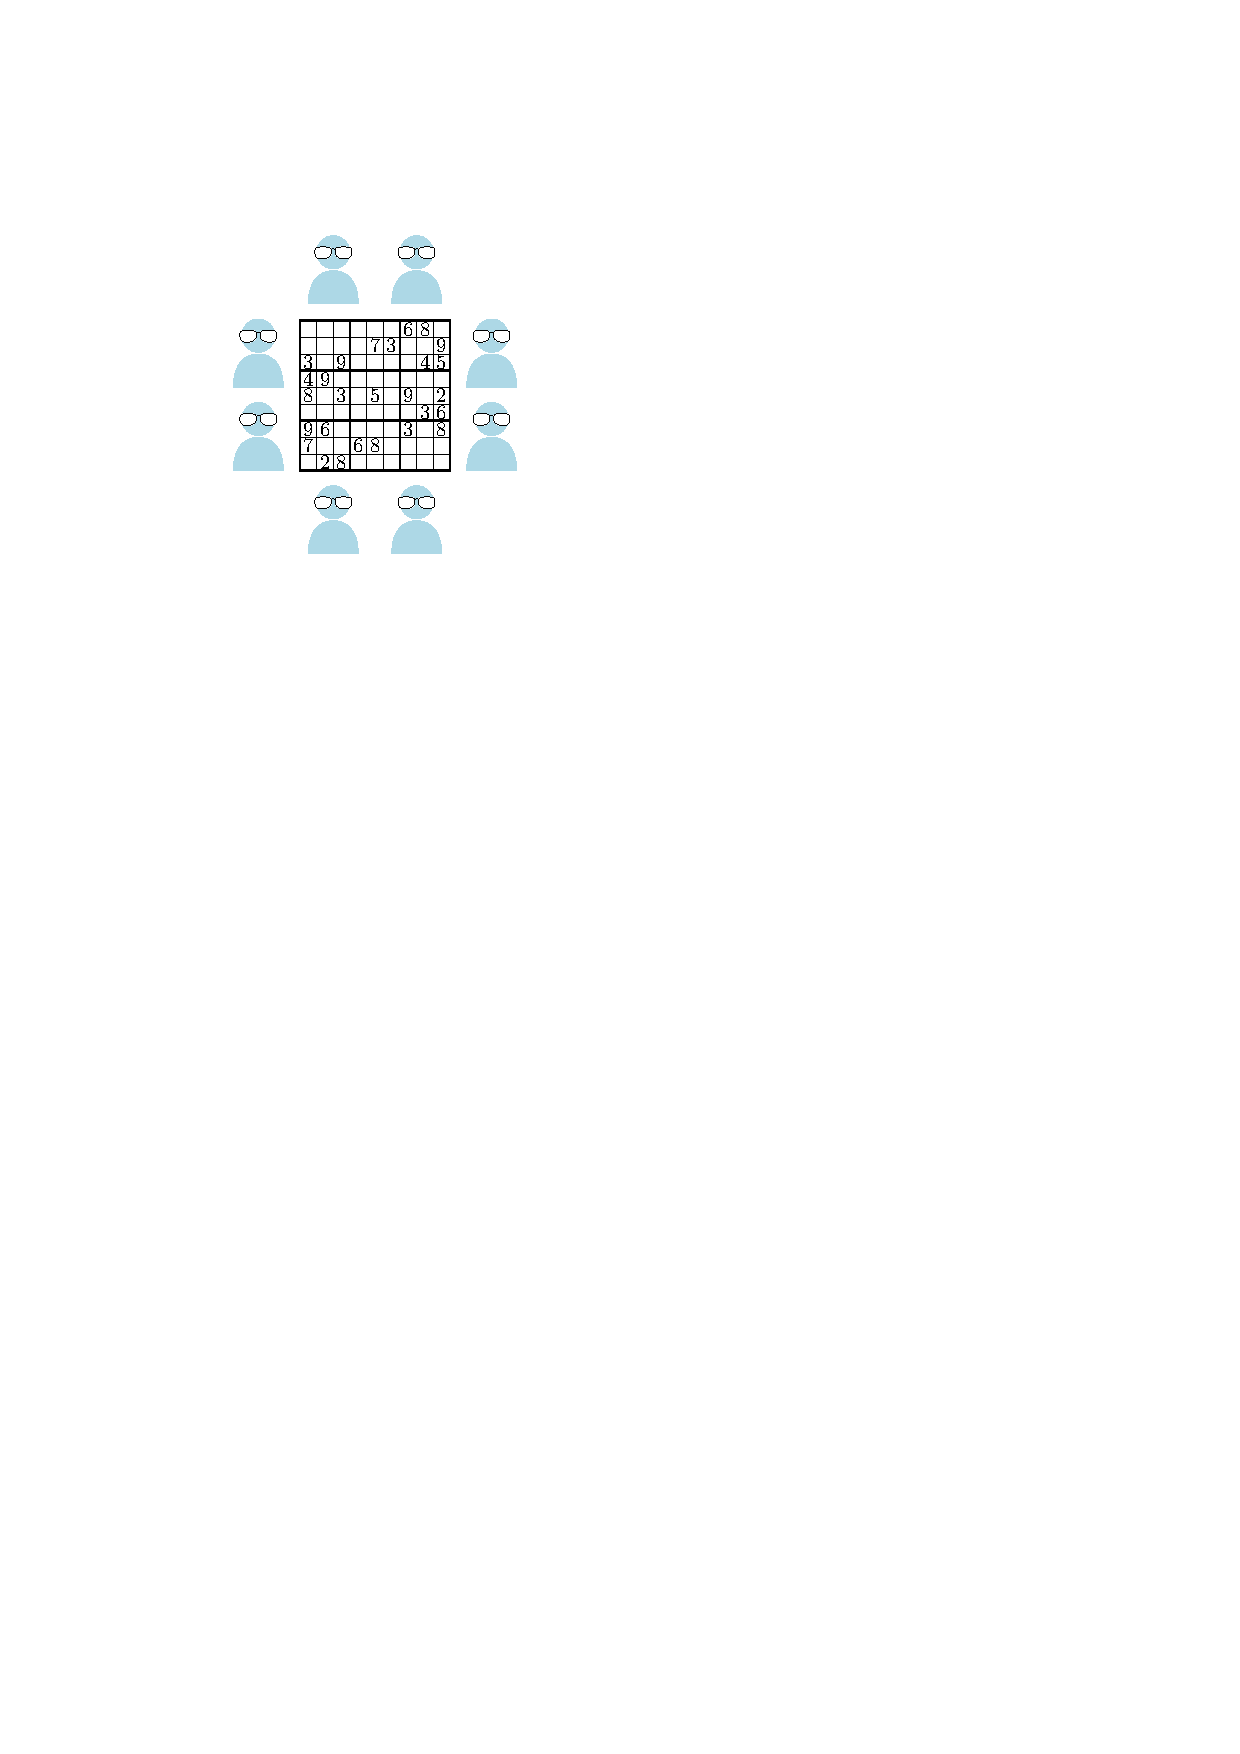
\includegraphics[width=10.8cm]{figures/l08/sudoku-1.pdf}	
	\end{minipage}
\end{frame}

\begin{frame}{Approach II: Pure Portfolio}
	\centering
	\only<1>{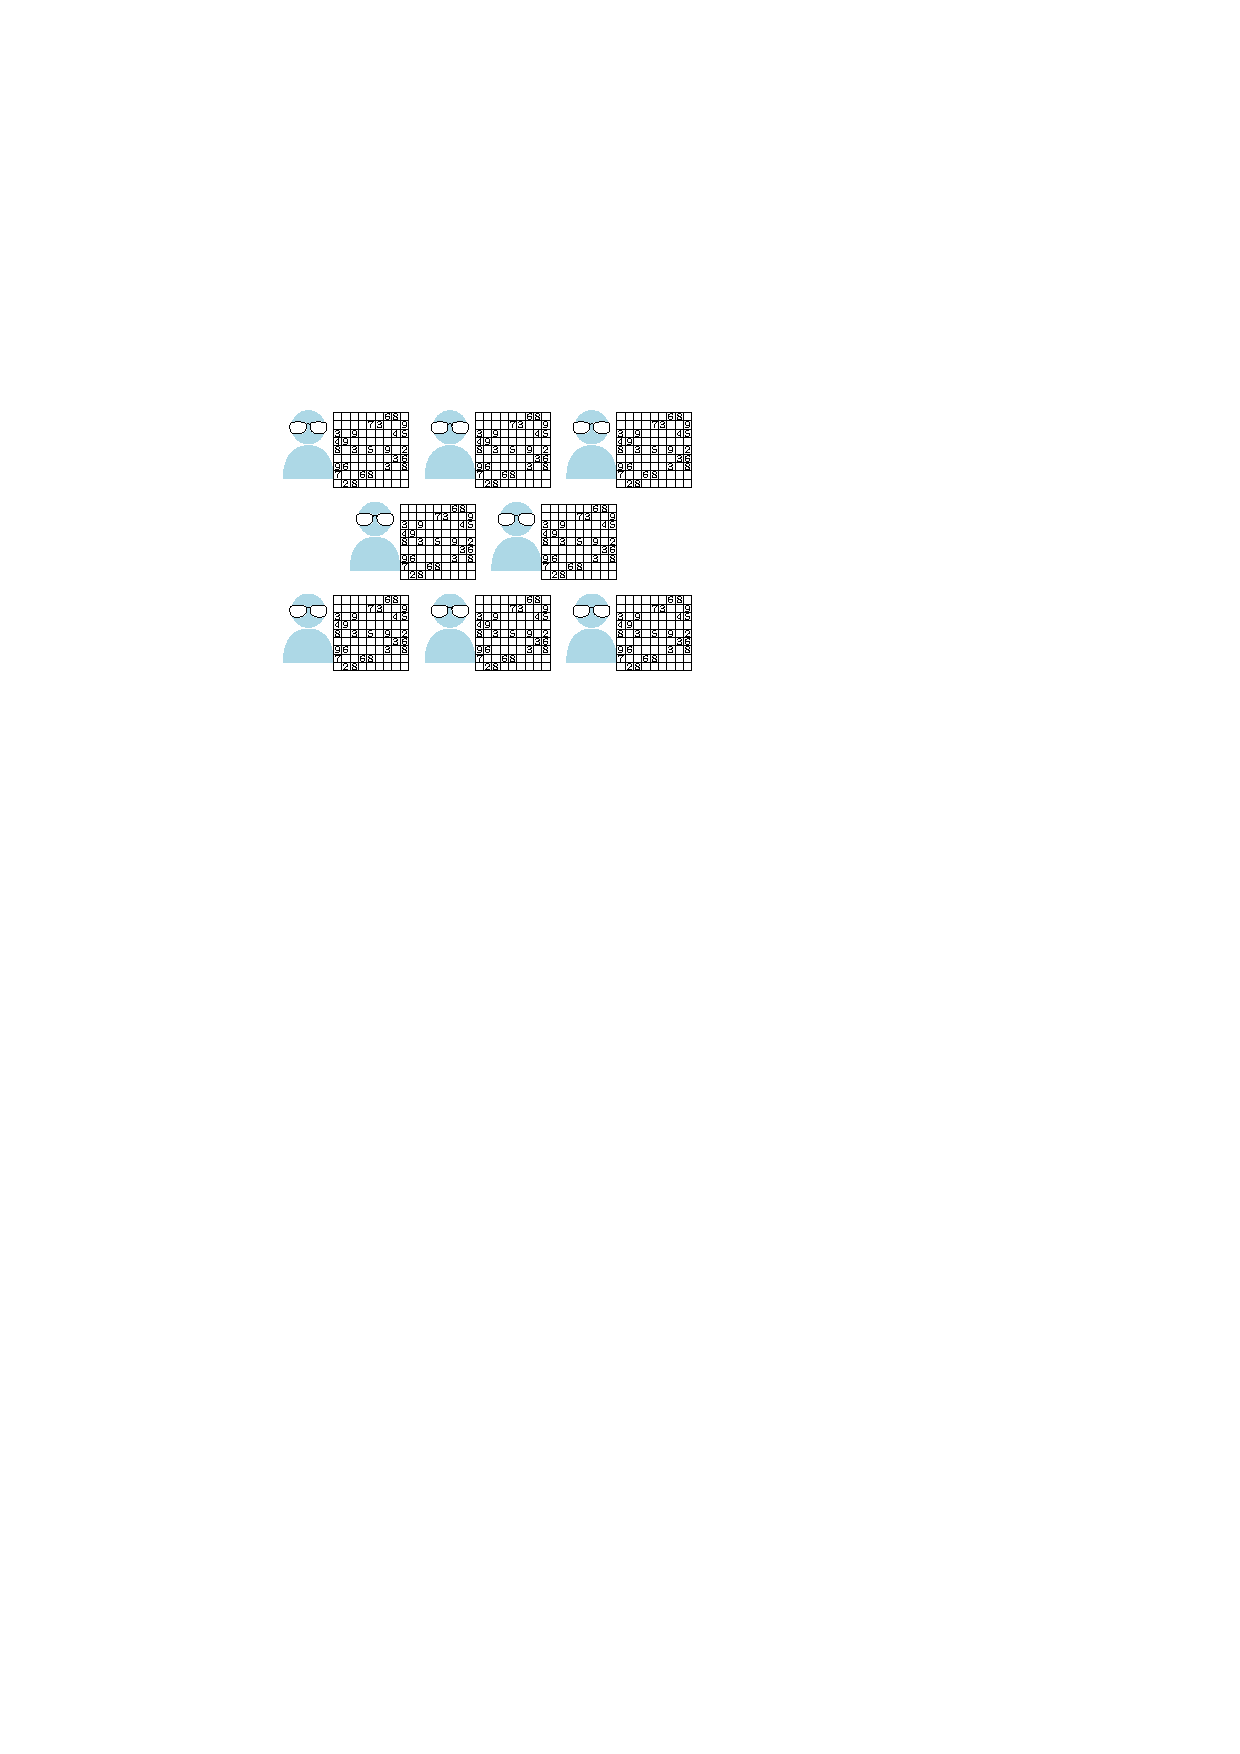
\includegraphics[width=19cm,page=1]{figures/l08/sudoku-2.pdf}}%
	\only<2>{\includegraphics[width=19cm,page=2]{figures/l08/sudoku-2.pdf}}%
	\only<3>{\includegraphics[width=19cm,page=3]{figures/l08/sudoku-2.pdf}}%	
\end{frame}

\begin{frame}{Pure Portfolio: Oracle view vs. Speedup view}
	\begin{blueblock}{Virtual Best Solver (VBS) / Oracle}
		Consider $n$ algorithms $A_1, \ldots, A_n$ where for each input $x$, algorithm $A_i$ has run time $T_{A_i}(x)$.\\
		The \highl{Virtual Best Solver} (VBS) for $A_1, \ldots, A_n$ has run time $T^*(x) = \min\{ T_{A_1}(x), \ldots, T_{A_n}(x) \}$.
	\end{blueblock}
	\pause
	\textbf{Optimist}: A pure portfolio \highl{simulates the VBS} using parallel processing!
	\begin{itemize}
		\item On idealized hardware, we \highl{``select'' best sequential solver} for each instance
	\end{itemize}
	\vspace*{0.5cm}
	\pause
	\begin{blueblock}{Parallel speedup~\cite{sanders2019sequential}}
		Given parallel algorithm $P$ and input $x$, the \highl{speedup} of $P$ is defined as $s_P(x) = T_Q(x) / T_P(x)$\\
		where $Q$ is the \highl{best available sequential algorithm}.
	\end{blueblock}
	\pause
	\textbf{Pessimist}: A pure portfolio \highlo{never achieves actual speedups}!
	\begin{itemize}
		\item There is always a sequential algorithm performing \highlo{at least as well}
		\item Consequence: \highlo{Not resource efficient}, \highlo{not scalable}
	\end{itemize}
\end{frame}

\begin{frame}{Pure SAT Portfolios}
	\begin{blueblock}{ppfolio: Winner of Parallel Track in the 2011 SAT Competition~\cite{roussel2012description}}
		\begin{itemize}
			\item Just a bash script combining the \highl{best sequential solvers from 2010}:\\
			\texttt{\~{}\$ ./solver1 f.cnf \& ./solver2 f.cnf \& ./solver3 f.cnf \& ./solver4 f.cnf}
			\item Bits by O. Roussel, the author of \texttt{ppfolio}:\\
			--- ``\textit{by definition the \highl{best solver on Earth}}''\\
			--- ``\textit{probably the \highlo{laziest and most stupid solver ever written}}''
		\end{itemize}
	\end{blueblock}
	\vspace*{0.2cm}
	\pause
	\begin{itemize}
		\item Rationale: Different solvers are designed differently, excel on different instances\\
		--- hope of \highl{orthogonal search behavior}
		\item Pure portfolios \highlo{no longer permitted} in SAT Competitions
	\end{itemize}
\end{frame}

\begin{frame}{Approach II+: Cooperative Portfolio}
	\centering
	\only<1>{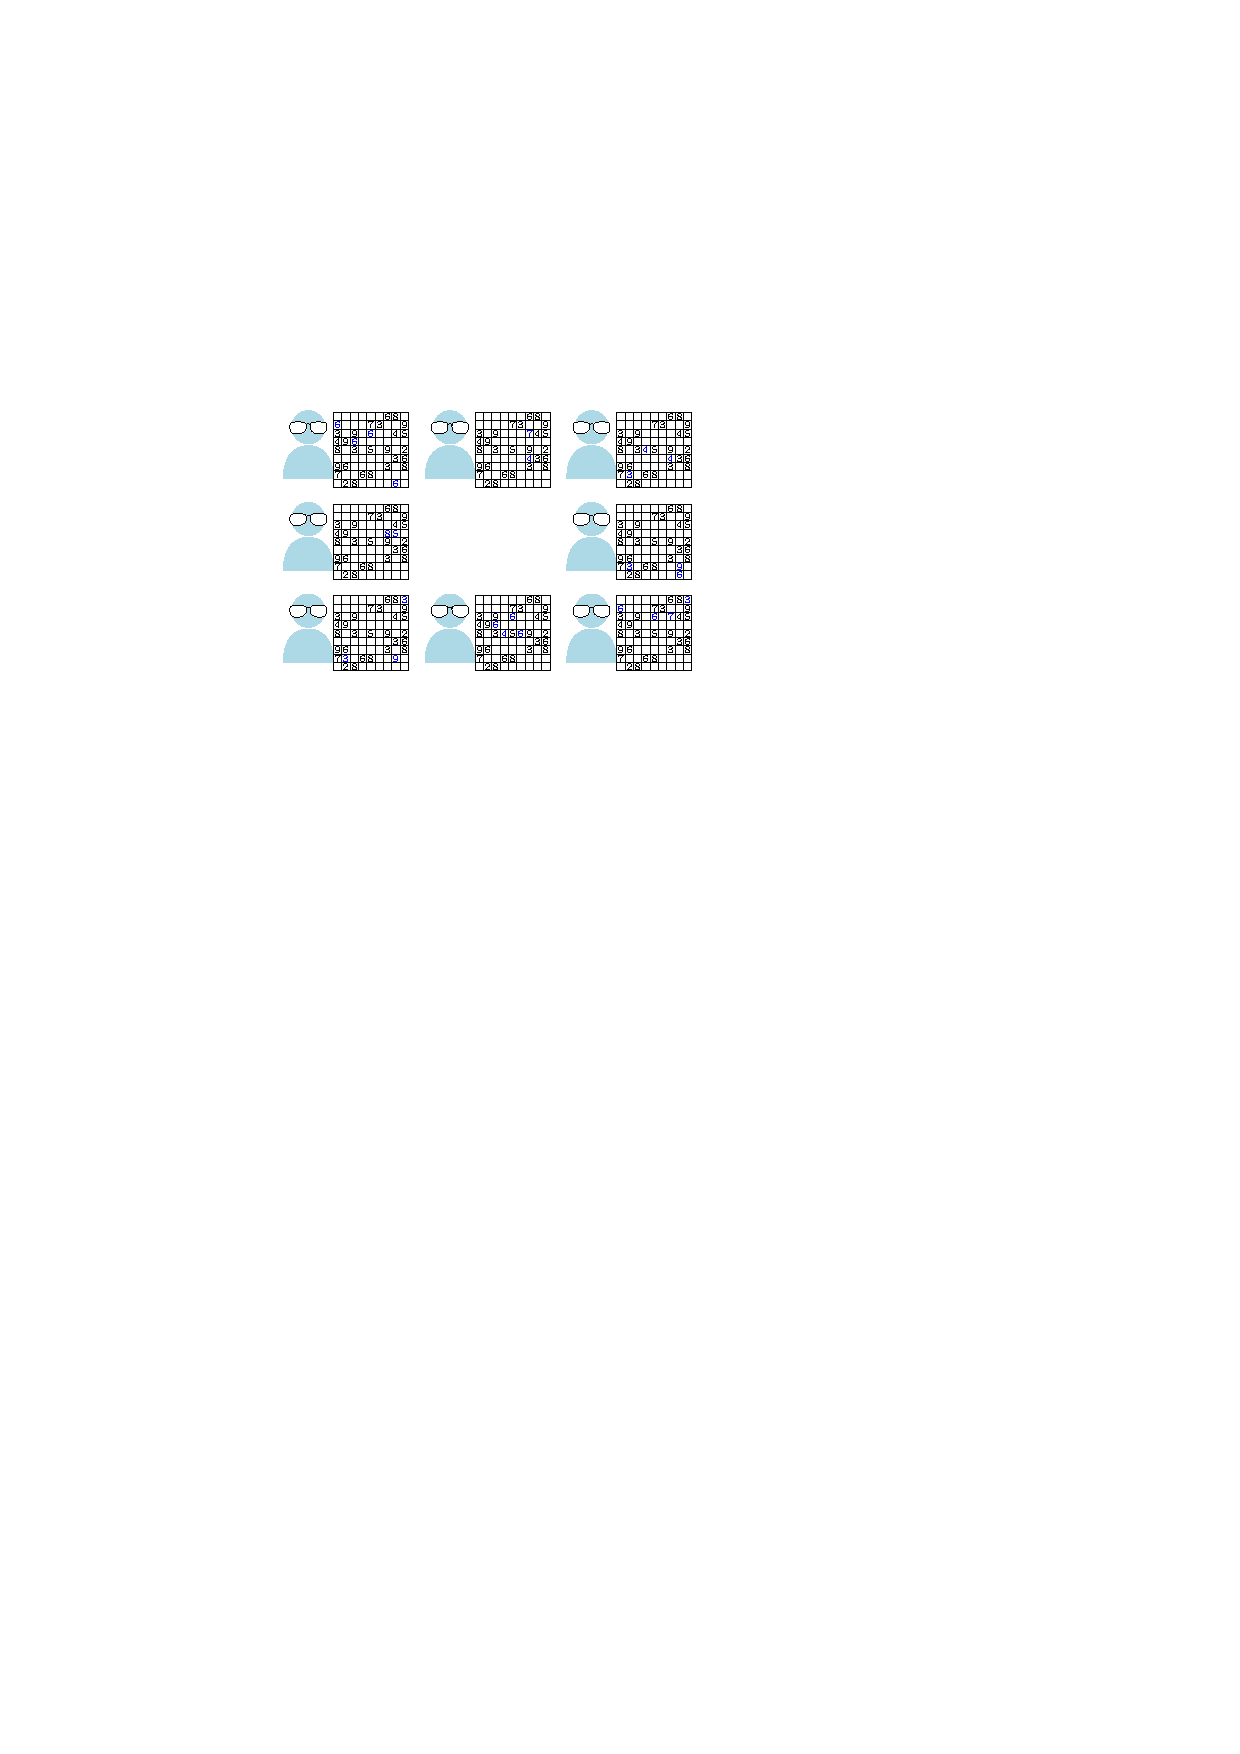
\includegraphics[page=1,width=19cm]{figures/l08/sudoku-3.pdf}}%
	\only<2>{\includegraphics[page=2,width=19cm]{figures/l08/sudoku-3.pdf}}%
	\only<3>{\includegraphics[page=3,width=19cm]{figures/l08/sudoku-3.pdf}}%
	\only<4>{\includegraphics[page=4,width=19cm]{figures/l08/sudoku-3.pdf}}%
\end{frame}

\begin{frame}{Cooperative Portfolio}
	\begin{blueblock}{Assembly of Nerds, enhanced}
		\begin{itemize}
			\item The experts periodically gather for \highl{brief standup meetings}
			\item Via some protocol, the experts exchange the \highl{most valuable insights gained} since the last meeting
			\item Solving continues	--- each expert may use the shared insights \highl{at their own discretion}
		\end{itemize}
	\end{blueblock}
	\vspace*{0.4cm}
	Equivalent to ``insights'' in SAT solving: \pause \textbf{learnt (conflict) clauses}
	\begin{itemize}
		\item Explored branch of search space --- \highl{safe to prune}
		\item Potential step for deriving \highlo{unsatisfiability}
		\item Result: \highl{Parallel search space pruning} procedure
	\end{itemize}
	\vspace*{0.4cm}
	\pause
	Combination of portfolio idea + clause exchanges: \textbf{Clause sharing portfolio solvers}
\end{frame}

\begin{frame}{Clause Sharing Portfolios: Design Space}
	\textbf{Portfolio considerations}
	\begin{itemize}
		\item \highl{Which sequential solvers} to employ?
		\item How to \highl{diversify} solvers?\\
		--- different \highl{search algorithms}, selection \highl{heuristics}, \highl{restart intervals}, \ldots\\
		--- different \highl{random seeds}, initial \highl{phases}, input \highl{permutations}, \ldots\\
	\end{itemize}
	\vspace*{0.3cm}
	\only<1>{
		\centering
		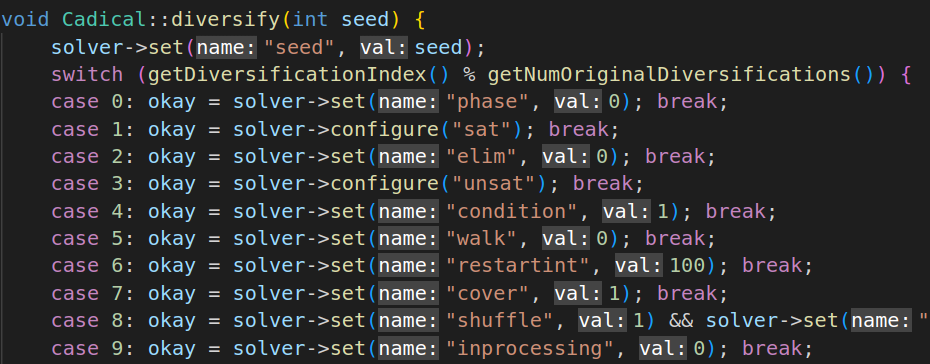
\includegraphics[width=0.6\textwidth]{figures/l08/code-diversification.png}	
	}
	\only<2->{
		\textbf{Clause exchange considerations}
		\begin{itemize}
			\item \highl{How often} to share? (immediate/eager? delayed/lazy? periodic?)
			\item \highl{How many clauses} to share? (fixed volume? fixed quality criteria?)
			\item \highl{Which clauses} to share? (shortest? lowest LBD?)
			\item \highl{How to implement} sharing? (all-to-all? leader-worker? some communication graph?)
	\end{itemize}}
\end{frame}

\begin{frame}{Early Clause Sharing Portfolios}
	
	\begin{blueblock}{ManySAT (Hamadi, Jabbour, and Sais 2009)~\cite{hamadi2010manysat}}
		\begin{itemize}
			\item Hand-crafted diversification of \highlo{four solver configurations}\\
			--- Restart policy, variable + polarity selection heuristic, \ldots
			\item Eager exchange of clauses of length $\leq 8$ via \highl{lockless queues}
		\end{itemize}
	\end{blueblock}
	\pause
	\begin{blueblock}{Plingeling (Biere 2010)~\cite{biere2010lingeling}}
		\begin{itemize}
			\item Portfolio over \highl{Lingeling configurations} (shared-memory parallelism)
			\item Lazy exchange of information over ``boss thread''\\
			--- 2010: \highl{Unit clauses} only
			\\
			--- 2011: Unit clauses + \highl{equivalences}
			\\
			--- Since 2013: Unit clauses + equivalences + \highl{clauses of length $\leq$ 40, LBD $\leq 8$}
			\item \highl{Best parallel solver} for many years
		\end{itemize}
	\end{blueblock}
\end{frame}

\begin{frame}{Massively parallel hardware?}
	\begin{blueblock}{Distributed computing, High-Performance Computing (HPC)}
		\begin{minipage}{0.6\textwidth}
			In \highl{distributed computing}, several \highl{machines}\\
			(with \highlo{no shared main memory}) run together.\\
			On each machine we run a number of \highl{processes},\\
			each of which runs on a number of \highl{cores}.\\
			Processes commonly communicate by \highl{exchanging messages}.
		\end{minipage}%
		\begin{minipage}{0.4\textwidth}
			\centering
			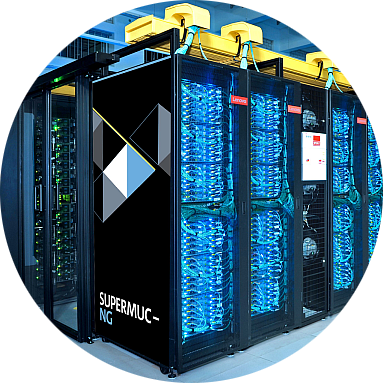
\includegraphics[width=0.3\textwidth]{figures/l08/supermuc-round.png}\\
			\unimp{SuperMUC-NG: 6\,336 nodes $\times$ 48 cores}
		\end{minipage}
	\end{blueblock}
	\vspace{0.3cm}
	\pause
	\textbf{Large distributed systems} (hundreds to thousands of cores) impose \highl{new requirements, challenges}:\\
	\vspace*{0.2cm}
	\begin{minipage}{0.7\textwidth}
		\begin{itemize}
			\item No shared memory --- \highl{communication protocols} required
			\item Diminishing returns due to \highlo{exhausted diversification} of solvers
			\pause
			\vspace*{1mm}
			\item Some exchange schemes are \highlo{conceptually not scalable}~\cite{ehlers2014communication}
			\begin{itemize}
				\item ``\highlo{Star graph}'': Master process collects, serves all exported clauses
				\item \highlo{Na{\"i}ve (quadratic) all-to-all exchange} of clauses
			\end{itemize}
			\item HPC schedulers, administrators, committees are used to \highl{regular,\\
				easily parallelizable code} with \highl{near-linear scaling}
		\end{itemize}
	\end{minipage}%
	\begin{minipage}{0.3\textwidth}
		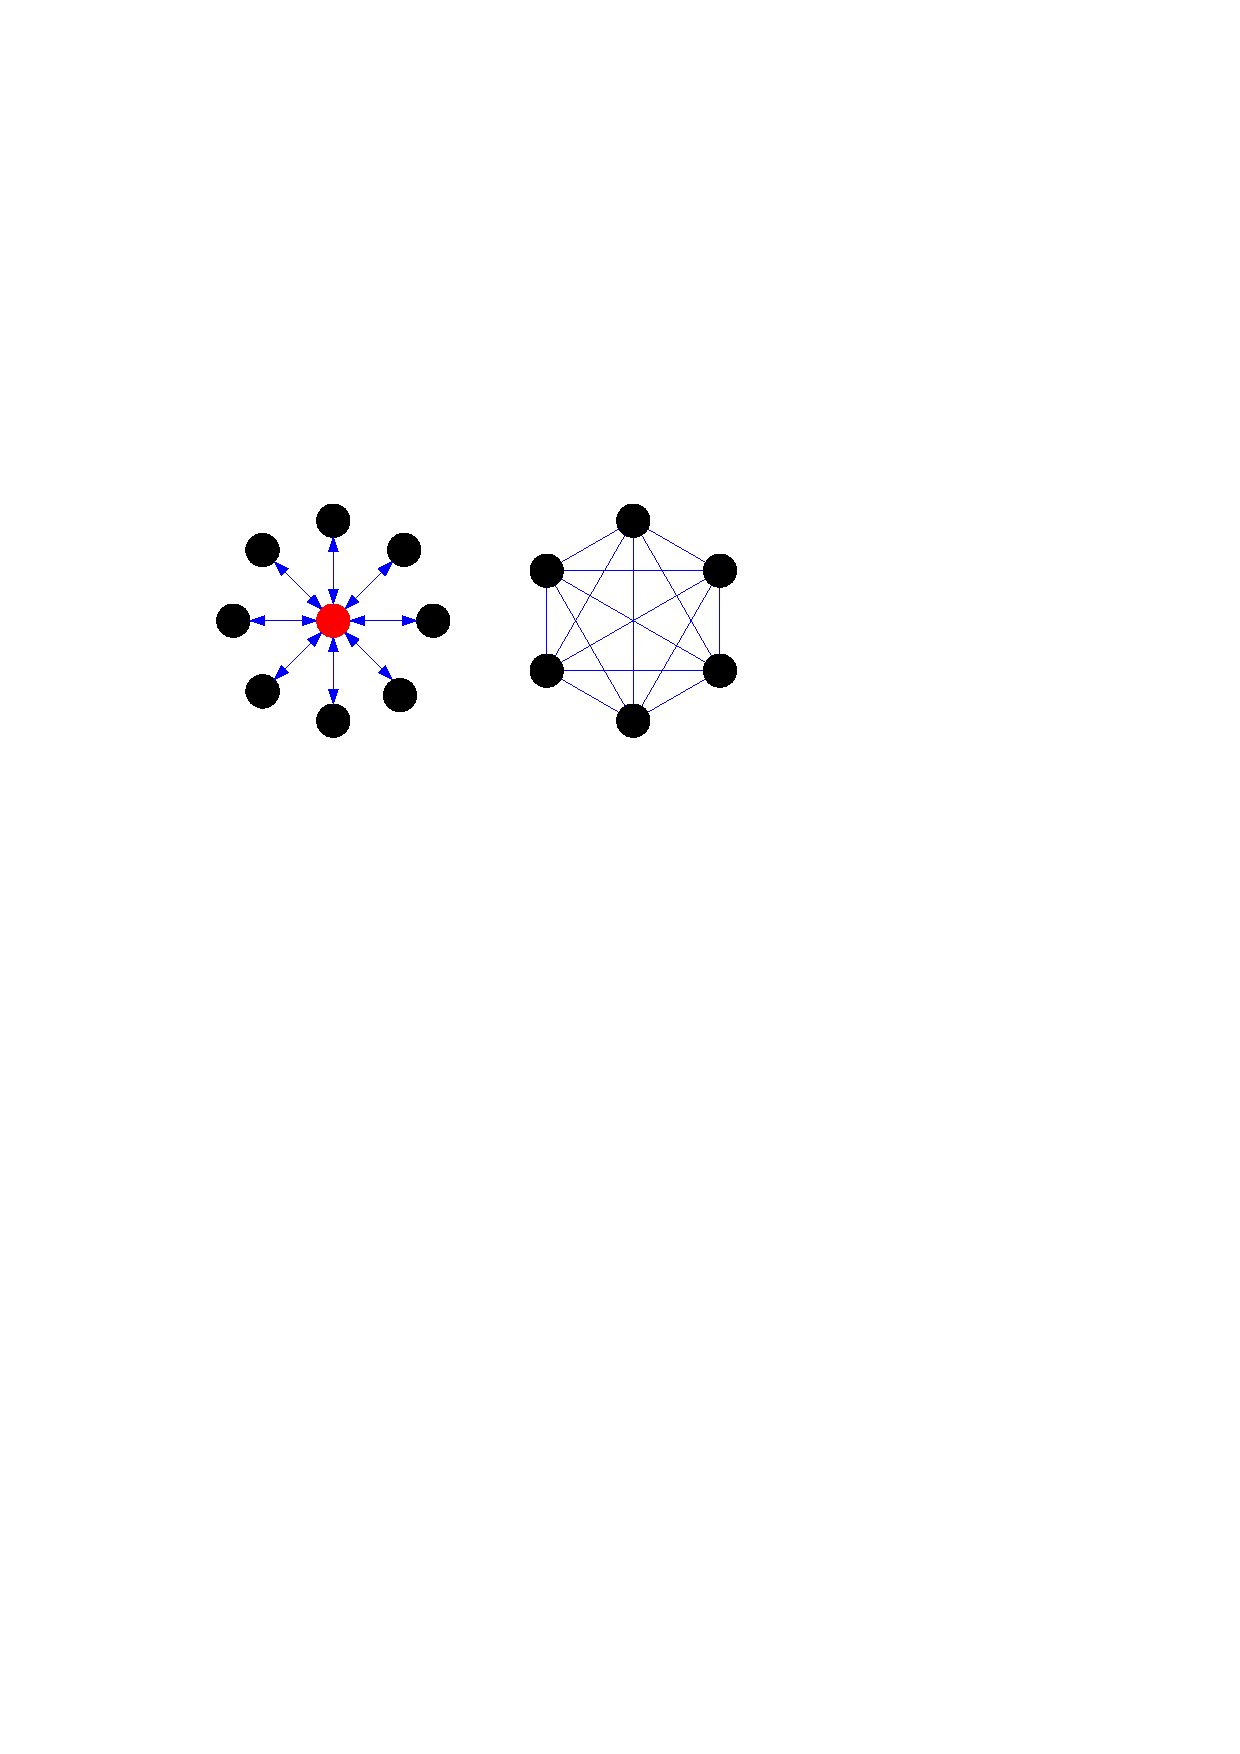
\includegraphics[width=\textwidth]{figures/l08/not-scalable-communication.pdf}
	\end{minipage}
\end{frame}

\begin{frame}{Massively parallel SAT portfolio}
	\begin{blueblock}{HordeSat (Balyo, Sanders, Sinz 2015)~\cite{balyo2015hordesat}}
		\begin{itemize}
			\item \highl{Decentralization}: No single leader node / process
			\item \highl{Two-level (``hybrid'') parallelization}\\
			--- One or several processes on each machine\\
			--- Multiple solver threads (+ communication thread) on each process
			%\item \highl{Modular solver interface}\\
			%--- Sequential solvers as interchangeable blackboxes\\
			%--- Small generic API to connect solvers
			%\item \highl{Overlapping search and communication}\\
			%--- Communication thread may block during collective operation\\
			%--- Solvers never wait, always continue solving
			\pause
			\iflecture{
				\item Diversification options:\\
				--- \highl{Native diversification} (set of hand-crafted solver configurations)\\
				--- Modifying some \highl{initial variable phases}\\
				--- Random seeds
			}
			\item Periodic \highl{all-to-all clause exchange}
		\end{itemize}
	\end{blueblock}
\end{frame}

\begin{frame}{Clause Exchange in HordeSat}
	\vspace*{-1cm}
	\begin{minipage}{0.51\textwidth}
		\begin{blueblock}{HordeSat's sharing logic}
			\vspace*{1.5mm}
			\begin{itemize}
				\item Only clauses with \highl{LBD $\leq 2$} are considered for sharing
				\begin{itemize}
					\item Constraint is lifted successively if processes under-produce
				\end{itemize}
				\item Solver threads write eligible clauses into shared buffer
				\vspace*{1.5mm}
				\item<2-> Each process' \highl{best clauses} are shared with everyone
				\begin{itemize}
					\item Limited to 1500 clause literals per process
				\end{itemize}
			\end{itemize}
			\uncover<2->{
			$\Rightarrow$ Concatenation of $p$ produced clause buffers
			\begin{itemize}
				\item Approximate, post-hoc \highl{filtering} of clauses
			\end{itemize}
			}
		\end{blueblock}
		\vspace*{4mm}
		\uncover<3->{
		\textbf{Issues:}
		\begin{itemize}
			\item Many (``high'' LBD) clauses are not shared but \highlo{discarded}
			\item \highlo{``Holes''} in buffer carrying no information
			\item \highlo{Duplicate} clauses
			\item Buffer grows \highl{proportionally} with \# proc.\\
			$\Rightarrow$ \highlo{Bottleneck} w.r.t.~communication, local work
		\end{itemize}
		}
	\end{minipage}\quad\quad%
	\begin{minipage}{0.44\textwidth}
		\centering
		\uncover<2->{
		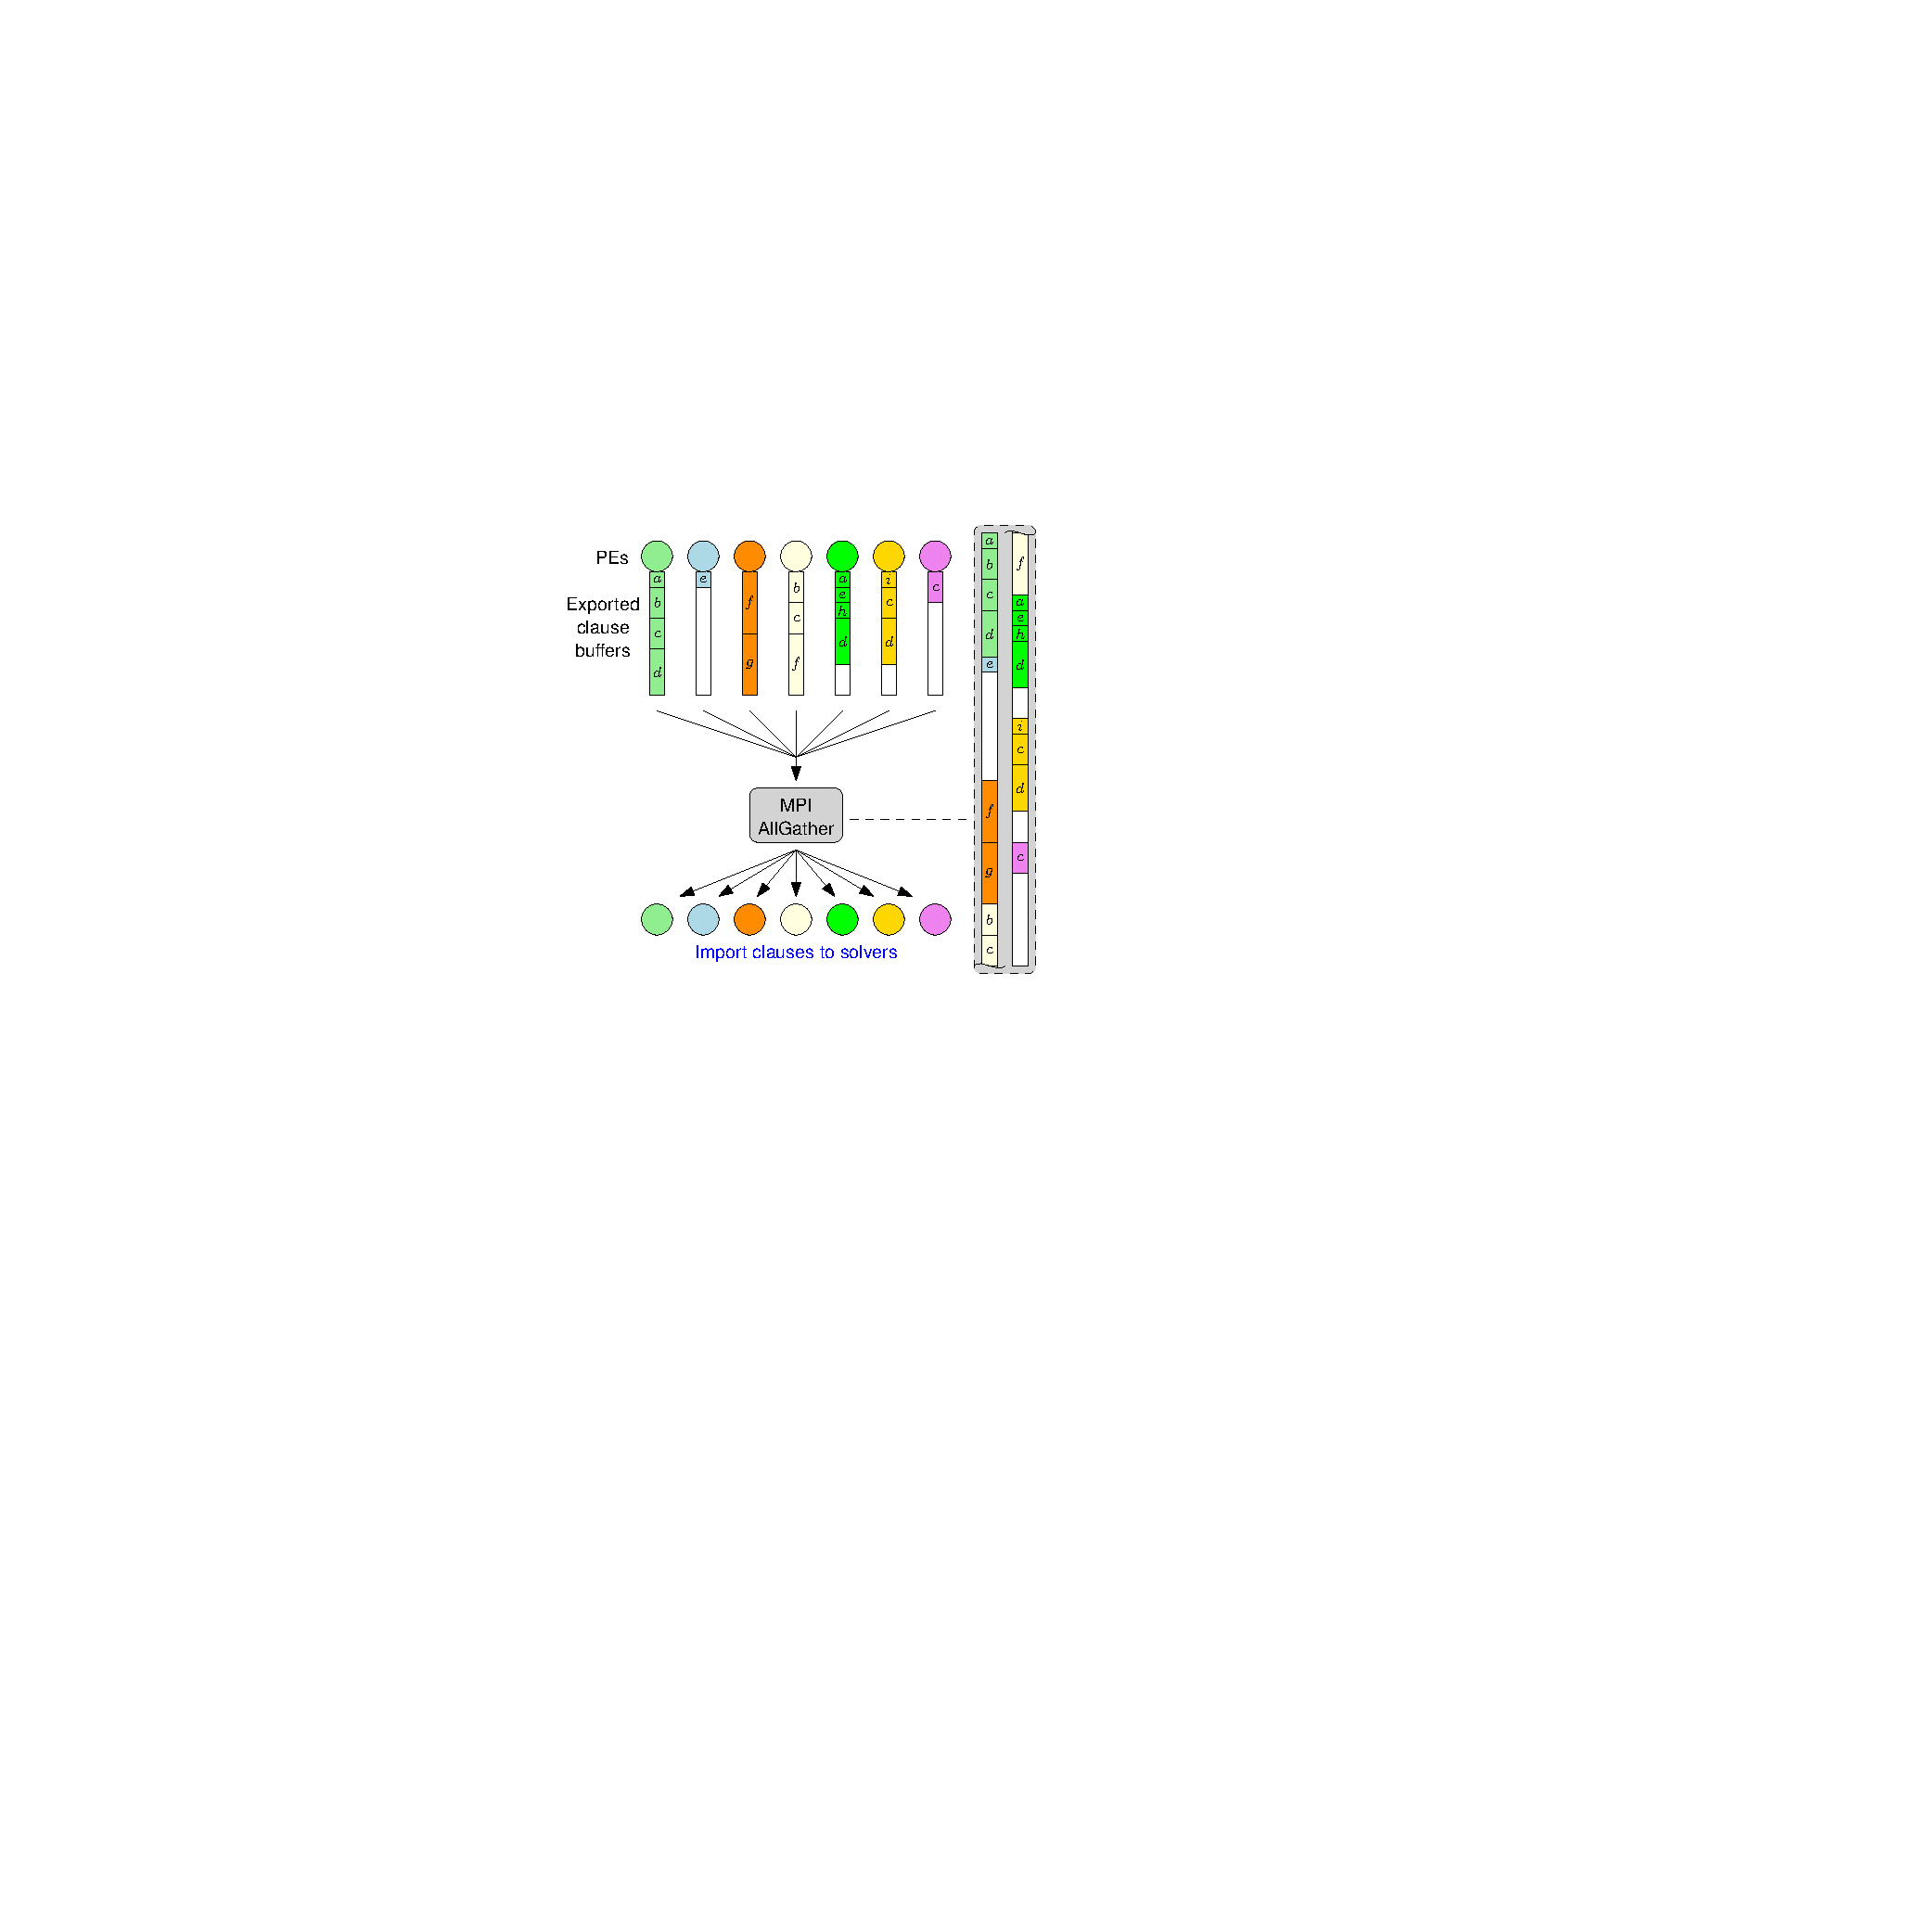
\includegraphics[width=\textwidth]{figures/l08/clause-sharing-horde.pdf}
		}
	\end{minipage}
\end{frame}

\begin{frame}{HordeSat: Results}
	\begin{minipage}{0.5\textwidth}
		\begin{itemize}
			\item \highl{Super-linear speedups} for individual instances\\
			= speedup \highl{$> c$} on $c$ cores!\quad\highlo{How?}\\[3mm]
			\iflecture{
				\pause
				--- SAT: ``\highl{NP luck}'' -- some solver got lucky\\
				--- UNSAT: \highl{distributed memory} accommodates\\
				\textcolor{white}{---} more clauses than any sequential solver\\
				--- General: \highl{sequential schedule} of parallel algorithm\\
				\textcolor{white}{---} may \highlo{outperform} sequential algorithm!
				\pause
			}
			\vspace*{2mm}
			\item Median speedup: 3 at 16 cores, \highlo{11.5 at 512 cores}\\
			--- \highl{Efficiency}: $11.5/512 \approx \highlo{2.2\%}$\\
			--- Deploying HordeSat is often \highlo{not worth it}
			\item No improvement \highlo{beyond $\approx$ 500 cores}
		\end{itemize}
	\end{minipage}%
	\begin{minipage}{0.5\textwidth}
		\ 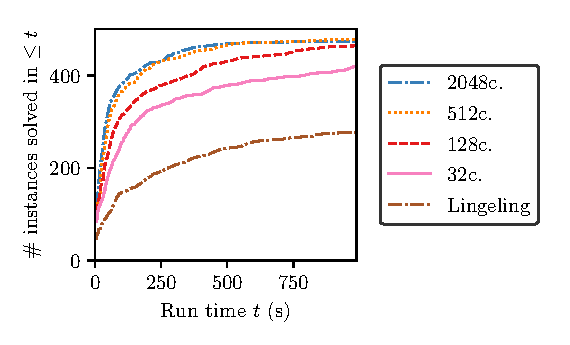
\includegraphics[width=1.05\textwidth]{figures/l08/hordescaling.pdf}\\
		\centering \unimp{Data extracted from HordeSat paper~\cite{balyo2015hordesat}}
	\end{minipage}%
\end{frame}

\begin{frame}{From HordeSat to MallobSat}
	\begin{block}{Research Question}
		How can we improve performance, (resource-)efficiency, and \highl{average response times}\\
		of SAT solving in \highl{modern distributed environments}?
	\end{block}
	\vspace*{0.3cm}
	%\renewcommand{\arraystretch}{1.2}
	\pause
	\begin{blueblock}{Result: Mallob}
		Mallob is a \highl{platform for SAT solving} (\emph{and other NP-hard problems}) with:
		\begin{itemize}
			\item multi-user, \highl{on-demand}, malleable scheduling and solving of \highl{many problems at once}~\cite{sanders2022decentralized}
			\item distributed SAT engine \textbf{MallobSat}: the HordeSat paradigm \highl{re-engineered and made efficient}~\cite{schreiber2021scalable}
			\item state-of-the-art SAT performance \highl{from dozens to thousands of cores}~\cite{schreiber2024mallobsat}
		\end{itemize}
	\end{blueblock}
	\vspace*{7mm}
	\begin{minipage}{0.5\textwidth}
		\centering
		
\includegraphics[width=11cm]{figures/l08/mallob-logo.jpg}
	\end{minipage}%
	\begin{minipage}{0.5\textwidth}
		\url{https://satres.kikit.kit.edu/research/mallob}
	\end{minipage}%
\end{frame}

%\begin{frame}{Outline: Lecture 2}
%	\textbf{Part A: Scalable SAT Solving}
%	\begin{itemize}
	%		\item Clause sharing and filtering
	%		\item Experimental results
	%		\item Solving many formulae at once
	%	\end{itemize}
%	\vspace*{0.3cm}
%	\textbf{Part B: Unsatisfiability Proofs}
%	\begin{itemize}
	%		\item Why? How?
	%		\item Sequential, then fully distributed approach
	%		\item Experimental results
	%	\end{itemize}
%\end{frame}


\begin{frame}{Design Decisions of \textsc{MallobSat}~\cite{schreiber2024mallobsat}}
	\begin{minipage}{0.45\textwidth}
		\begin{itemize}
			\item \textbf{Fundament:} \textsc{HordeSat}\\
			%\begin{itemize}
			{
				-- Two-level \highl{hybrid parallelization}\\
				%-- \highl{Modular solver interface}\\
				-- \highl{Periodic all-to-all} clause sharing}
			%\end{itemize}
			%\item<2-> Process layout \highl{faithful to hardware at hand}\\
			%{\small -- one SAT process per CPU socket}
			%\item<2-> Purely \highl{asynchronous communication}
			\item<2-> Fix a certain \highl{sharing volume}, spend it on\\
			the \highl{globally most useful \textbf{distinct} clauses}
			\item<3-> Prioritize clauses by \highl{clause length} over \highlo{LBD}\\
			-- \highl{At all stages!} Also in export / import buffering
			%\begin{itemize}
			%{\small -- LBD found by solver A \highlo{not necessarily\\
					%\phantom{--} meaningful} for solver B!}
			%\end{itemize}
			\item<4-> Minimize \highl{clause turnaround times}
			\item<5-> Support \highlo{fluctuating workers} (\highl{\textit{malleability}})
		\end{itemize}
	\end{minipage}\quad\quad%
	\begin{minipage}{0.47\textwidth}
		\centering
		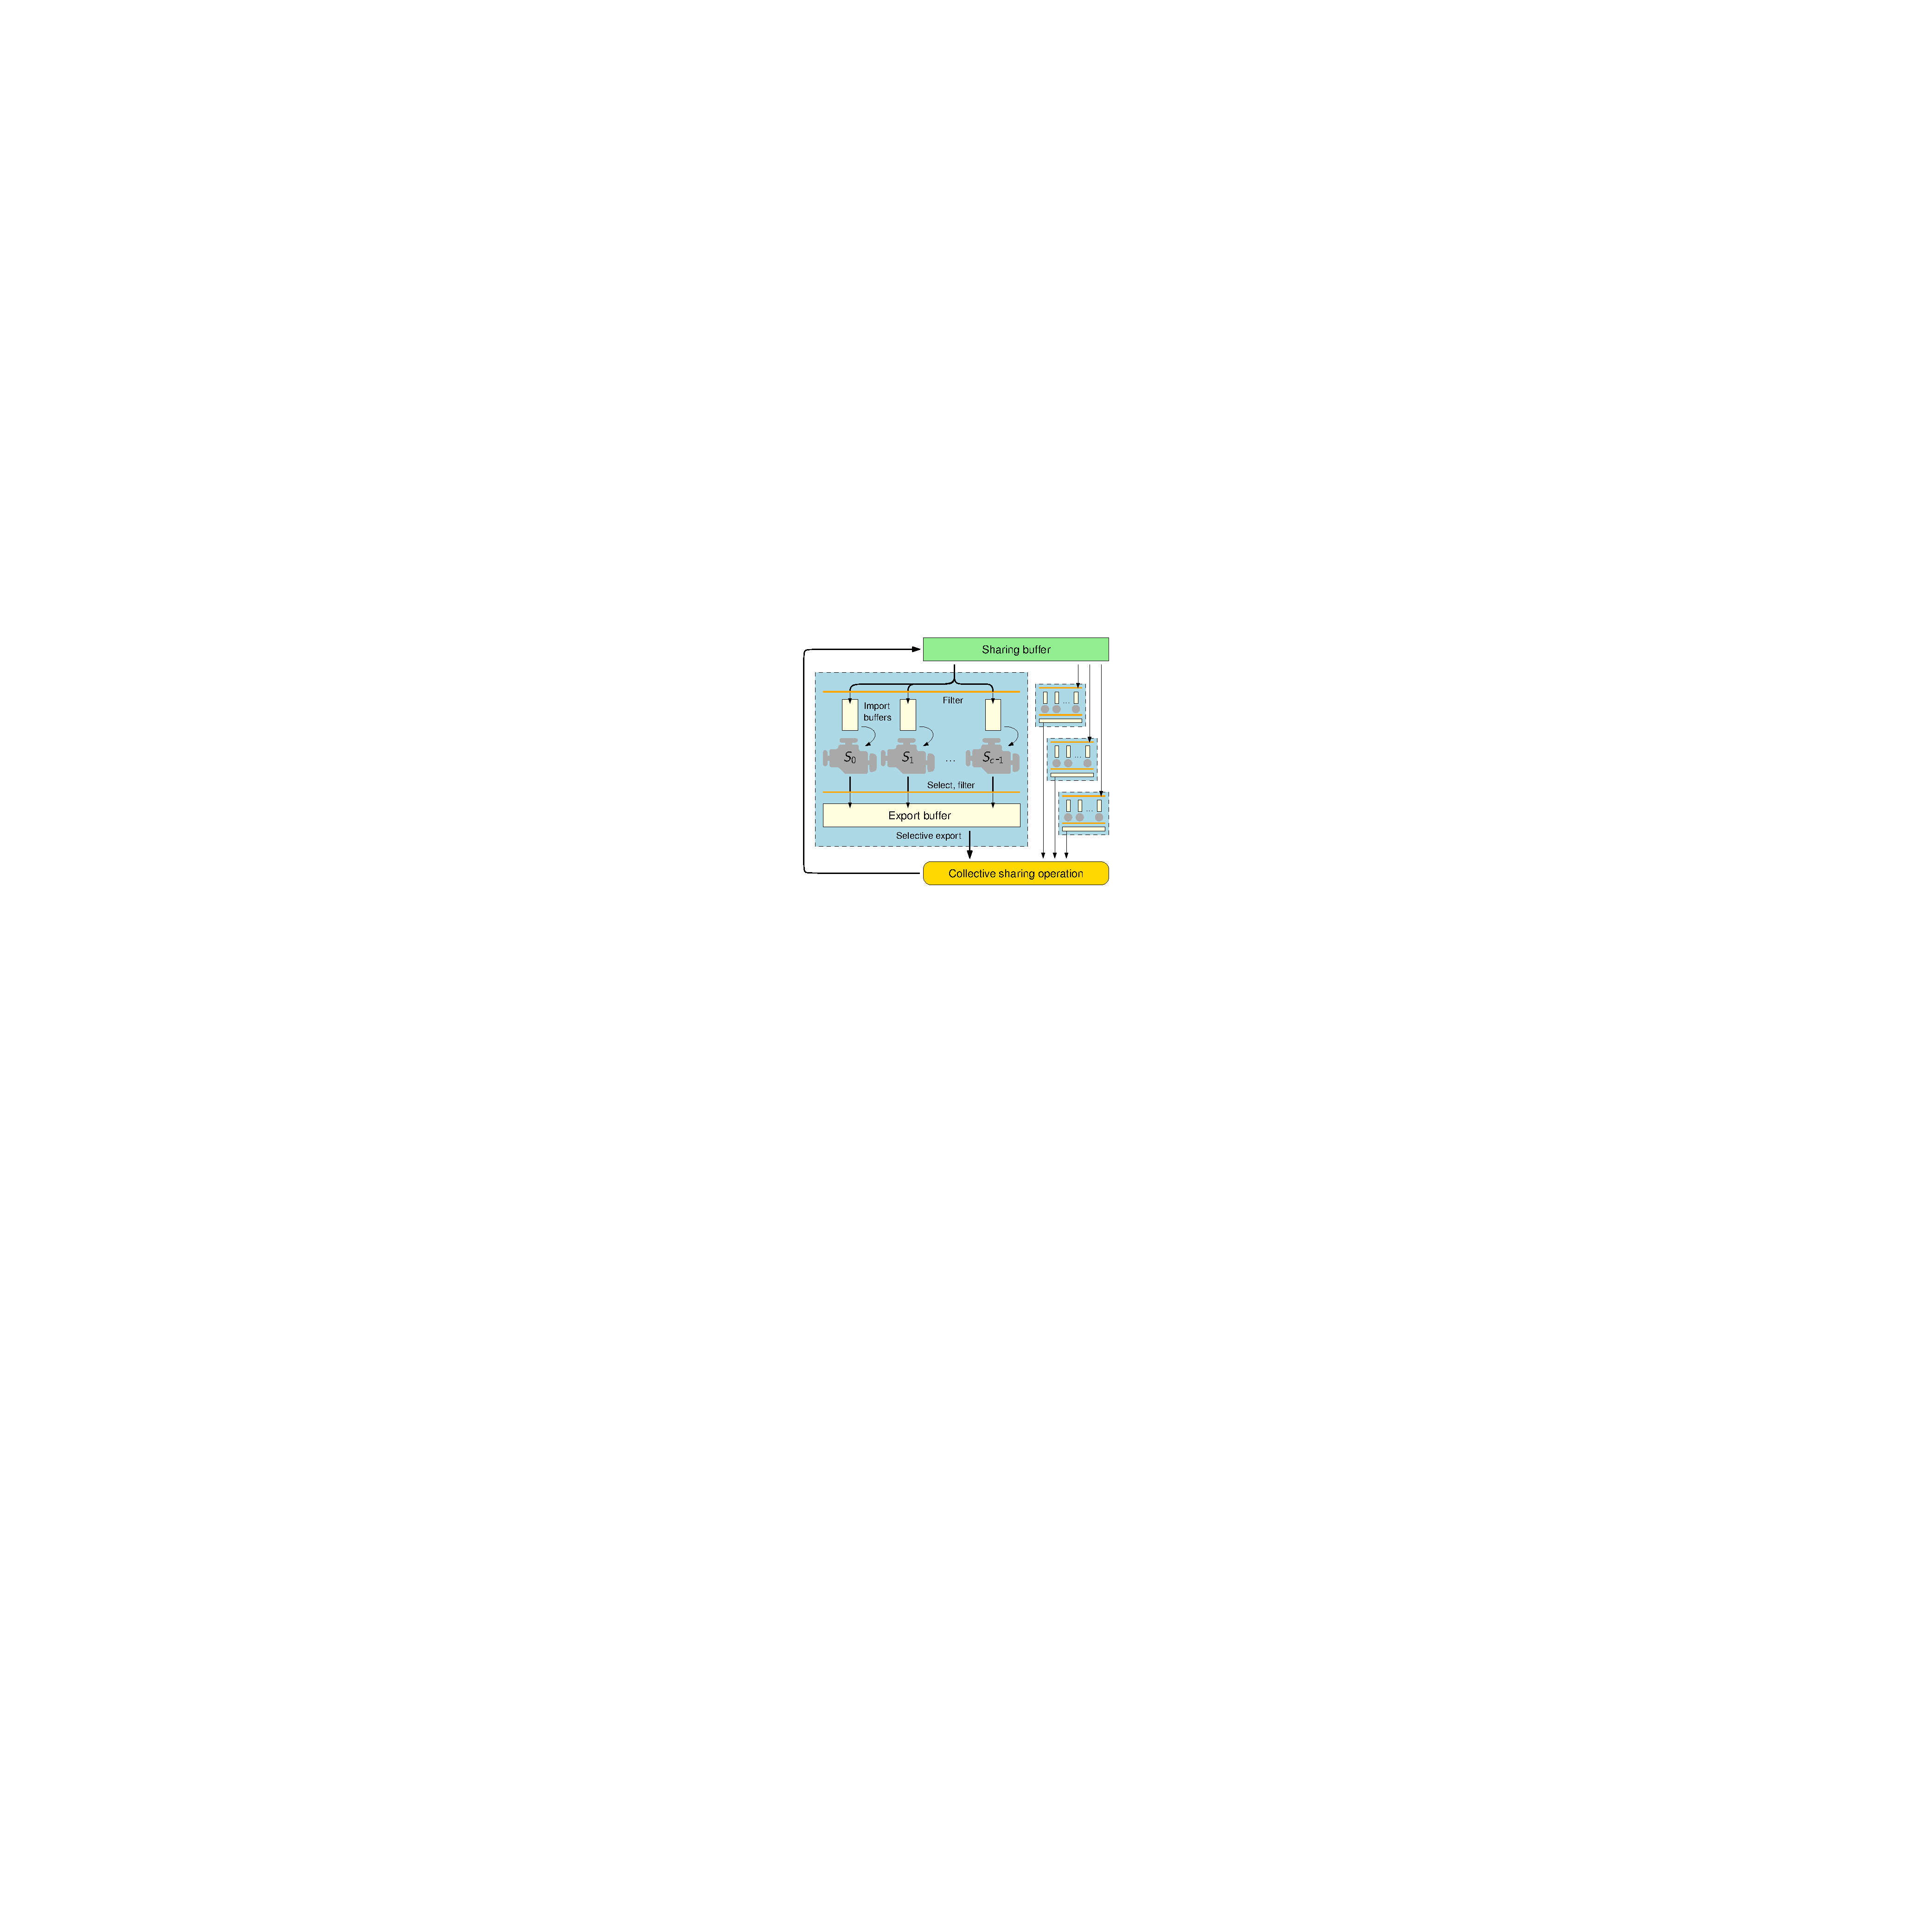
\includegraphics[width=\textwidth]{figures/l08/clause-sharing-overview.pdf}		
	\end{minipage}%
\end{frame}

\begin{frame}{Clause Exchange in Mallob~\cite{schreiber2024mallobsat}}
	\begin{minipage}{0.43\textwidth}
		\textbf{Custom collective operation}
		\begin{itemize}
			\item Aggregate information along\\
			\highl{binary tree of processors}
			\item \highl{Detect duplicates} during merge
			\item Result is of \highl{compact shape}
			\item \highl{Sublinear} buffer size growth:\\
			\highlo{Discard longest clauses} as necessary
		\end{itemize}
		
		\uncover<5>{
			\vspace*{5mm}
			\begin{blueblock}{Observations}
				\begin{itemize}
					\item Clause needs to meet \highl{global quality threshold} to be shared successfully
					\item Quality threshold \highl{adapts to state of solving}
				\end{itemize}
			\end{blueblock}
		}
	\end{minipage}\quad\quad%
	\begin{minipage}{0.5\textwidth}
		\centering
		\only<1>{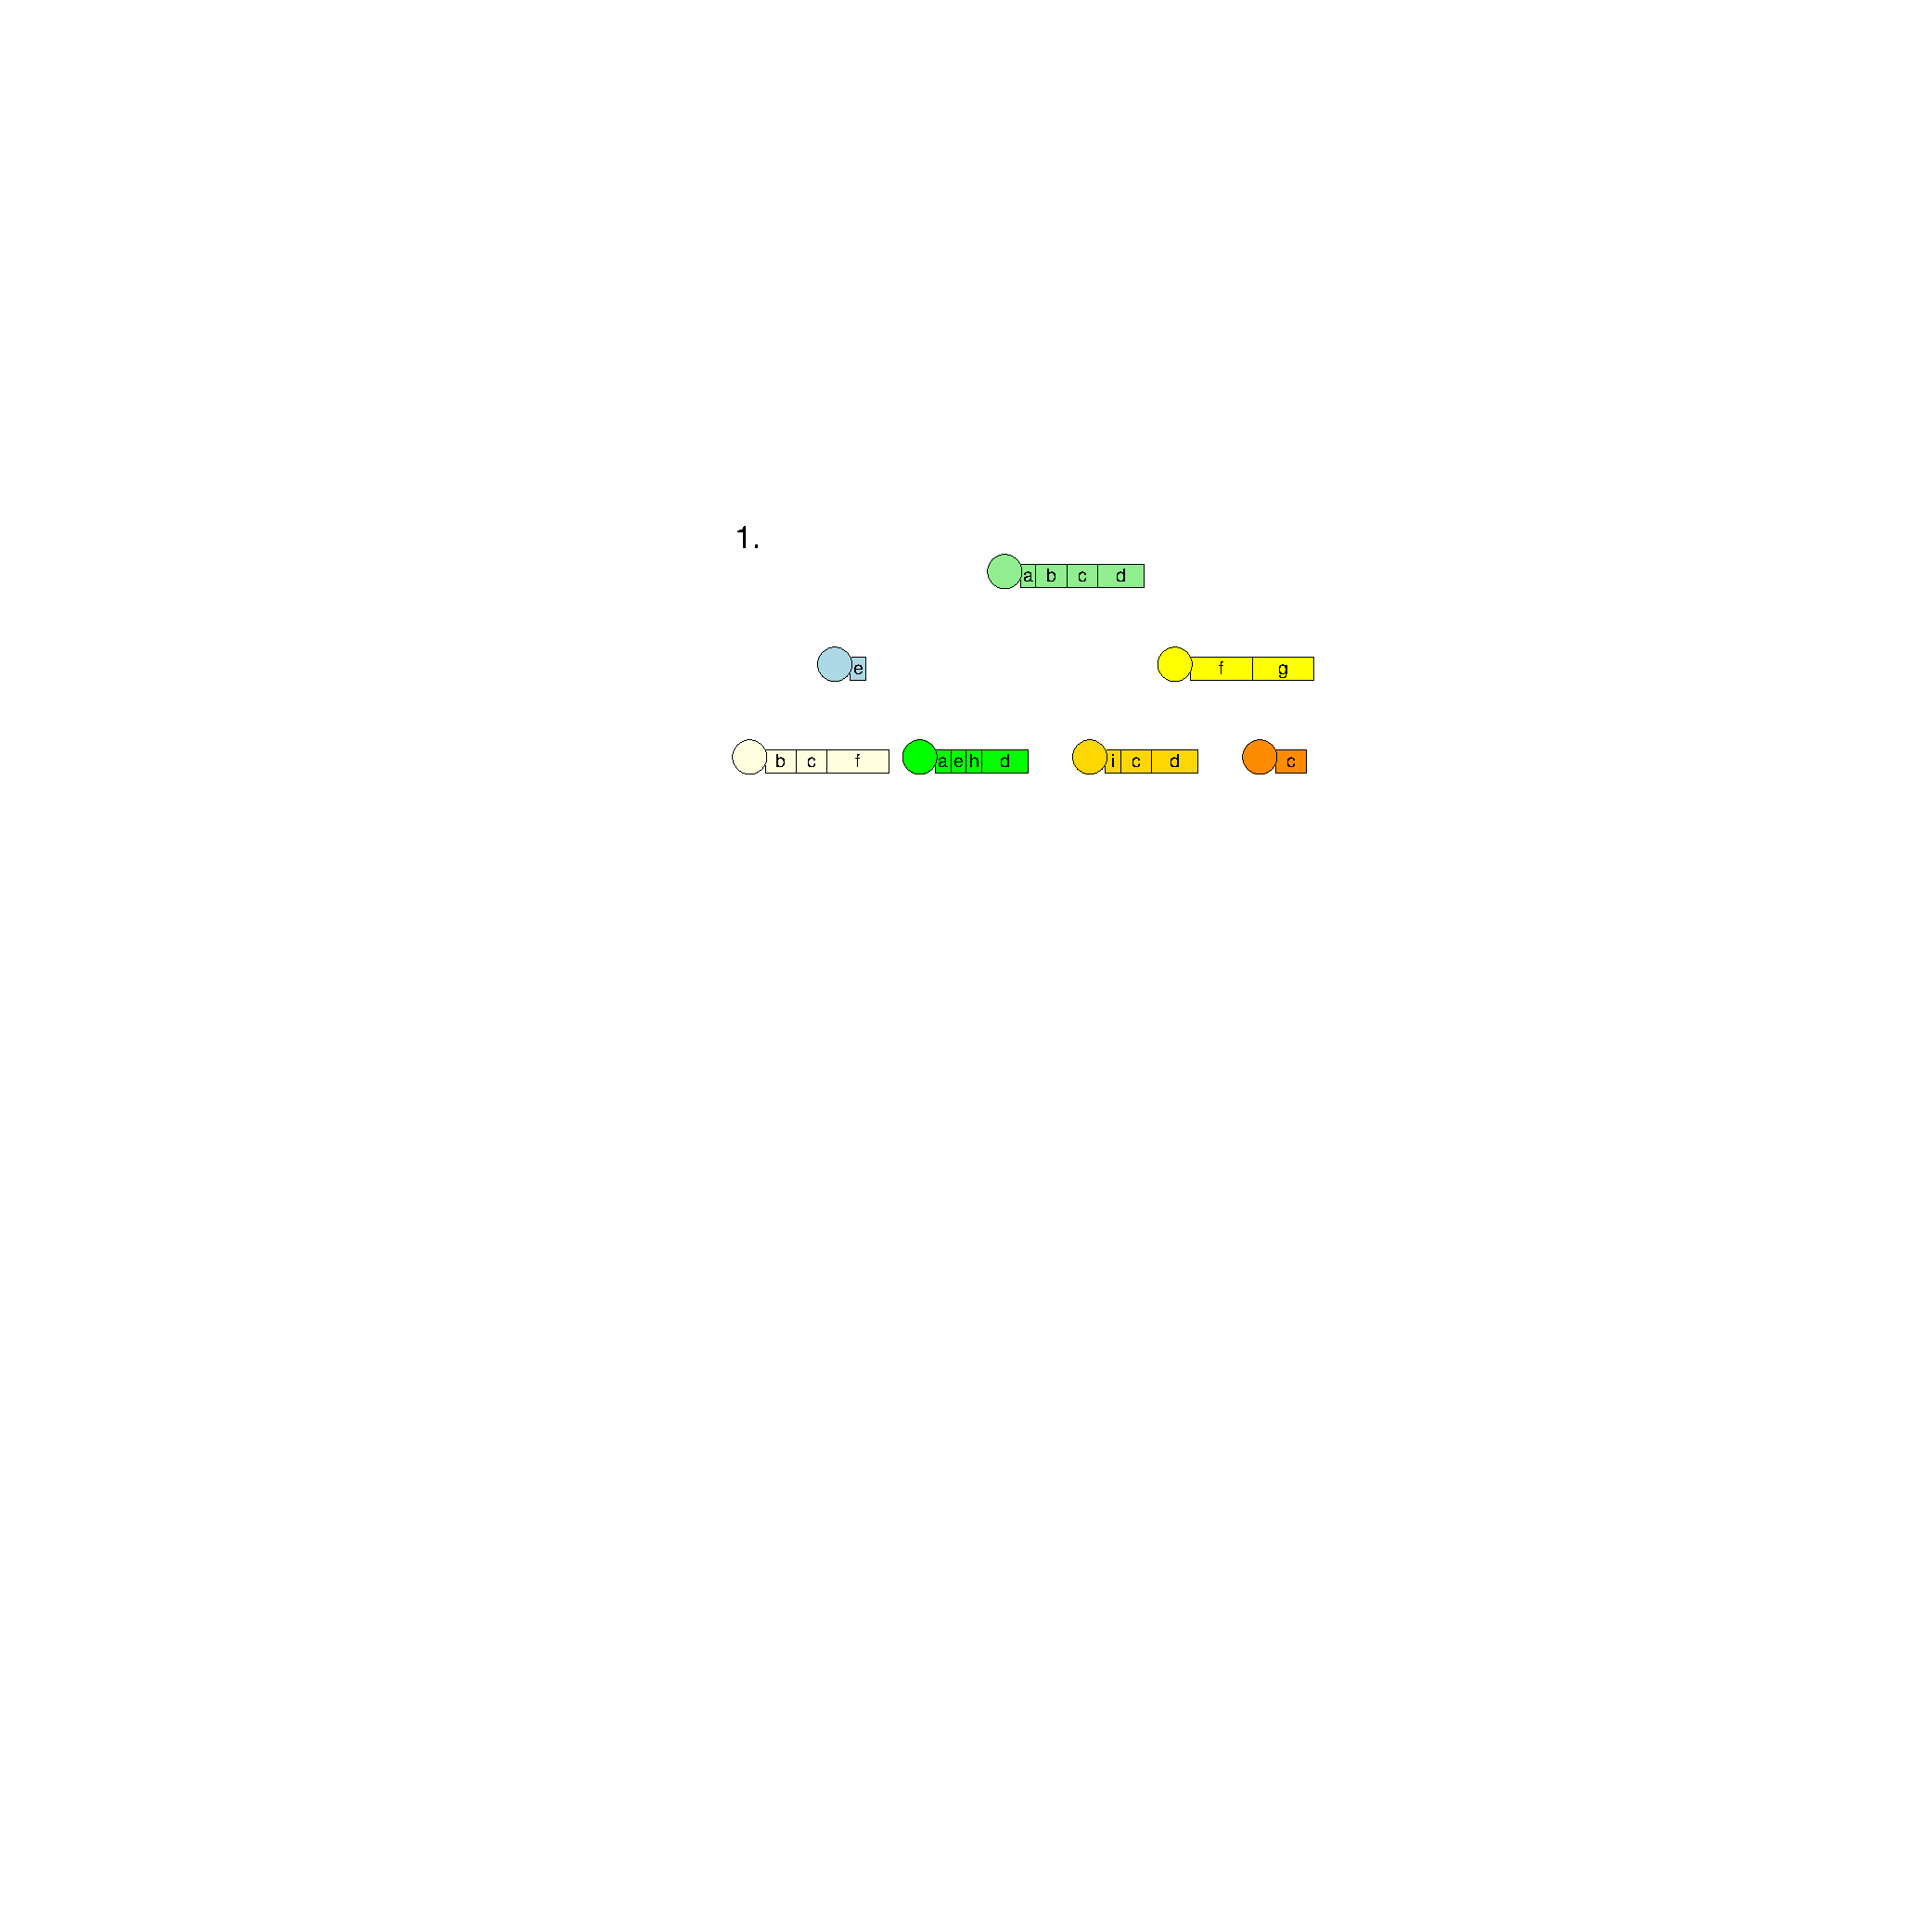
\includegraphics[width=\textwidth,page=1]{figures/l08/clause-sharing-mallob.pdf}}%
		\only<2>{\includegraphics[width=\textwidth,page=2]{figures/l08/clause-sharing-mallob.pdf}}%
		\only<3>{\includegraphics[width=\textwidth,page=3]{figures/l08/clause-sharing-mallob.pdf}}%
		\only<4->{\includegraphics[width=\textwidth,page=4]{figures/l08/clause-sharing-mallob.pdf}}%
	\end{minipage}
\end{frame}

\begin{frame}{Clause Filtering}
	\begin{minipage}{0.45\textwidth}
		\begin{blueblock}{The Problem}
			Given a \highl{shared clause} $c$ and a solver $S$, decide if\\
			$S$ has \highl{received or produced} $c$ before (recently).
		\end{blueblock}
		\vspace*{0.1cm}
		\textbf{Previously:}~\cite{balyo2015hordesat,schreiber2021scalable}
		\begin{itemize}
			\item Bloom filters: \highl{fixed size}, risk of \highlo{false positives}
			%\item Option for periodic clearing of filters
		\end{itemize}
		\vspace*{0.1cm}
		\pause
		\textbf{Mallob'22+:} \highl{Exact distributed filter}~\cite{schreiber2024mallobsat}
		\begin{itemize}
			\item Process $p$ remembers clauses \highl{it exported itself}\\
			and \highl{tags their producing solver(s)}
			\pause
			\item Aggregate bit vector $v$ where \highl{$v[i] := \bigvee_{\!p}\ (p\ \text{remembers}\ c_i)$}
			\item Only import clauses $c_i$ for which $v[i] =$ \texttt{false}
			\item<4-> Use producer data to prevent \highlo{mirroring clauses back} to their producer(s)
		\end{itemize}
	\end{minipage}\quad\quad%
	\begin{minipage}{0.48\textwidth}
		\only<1>{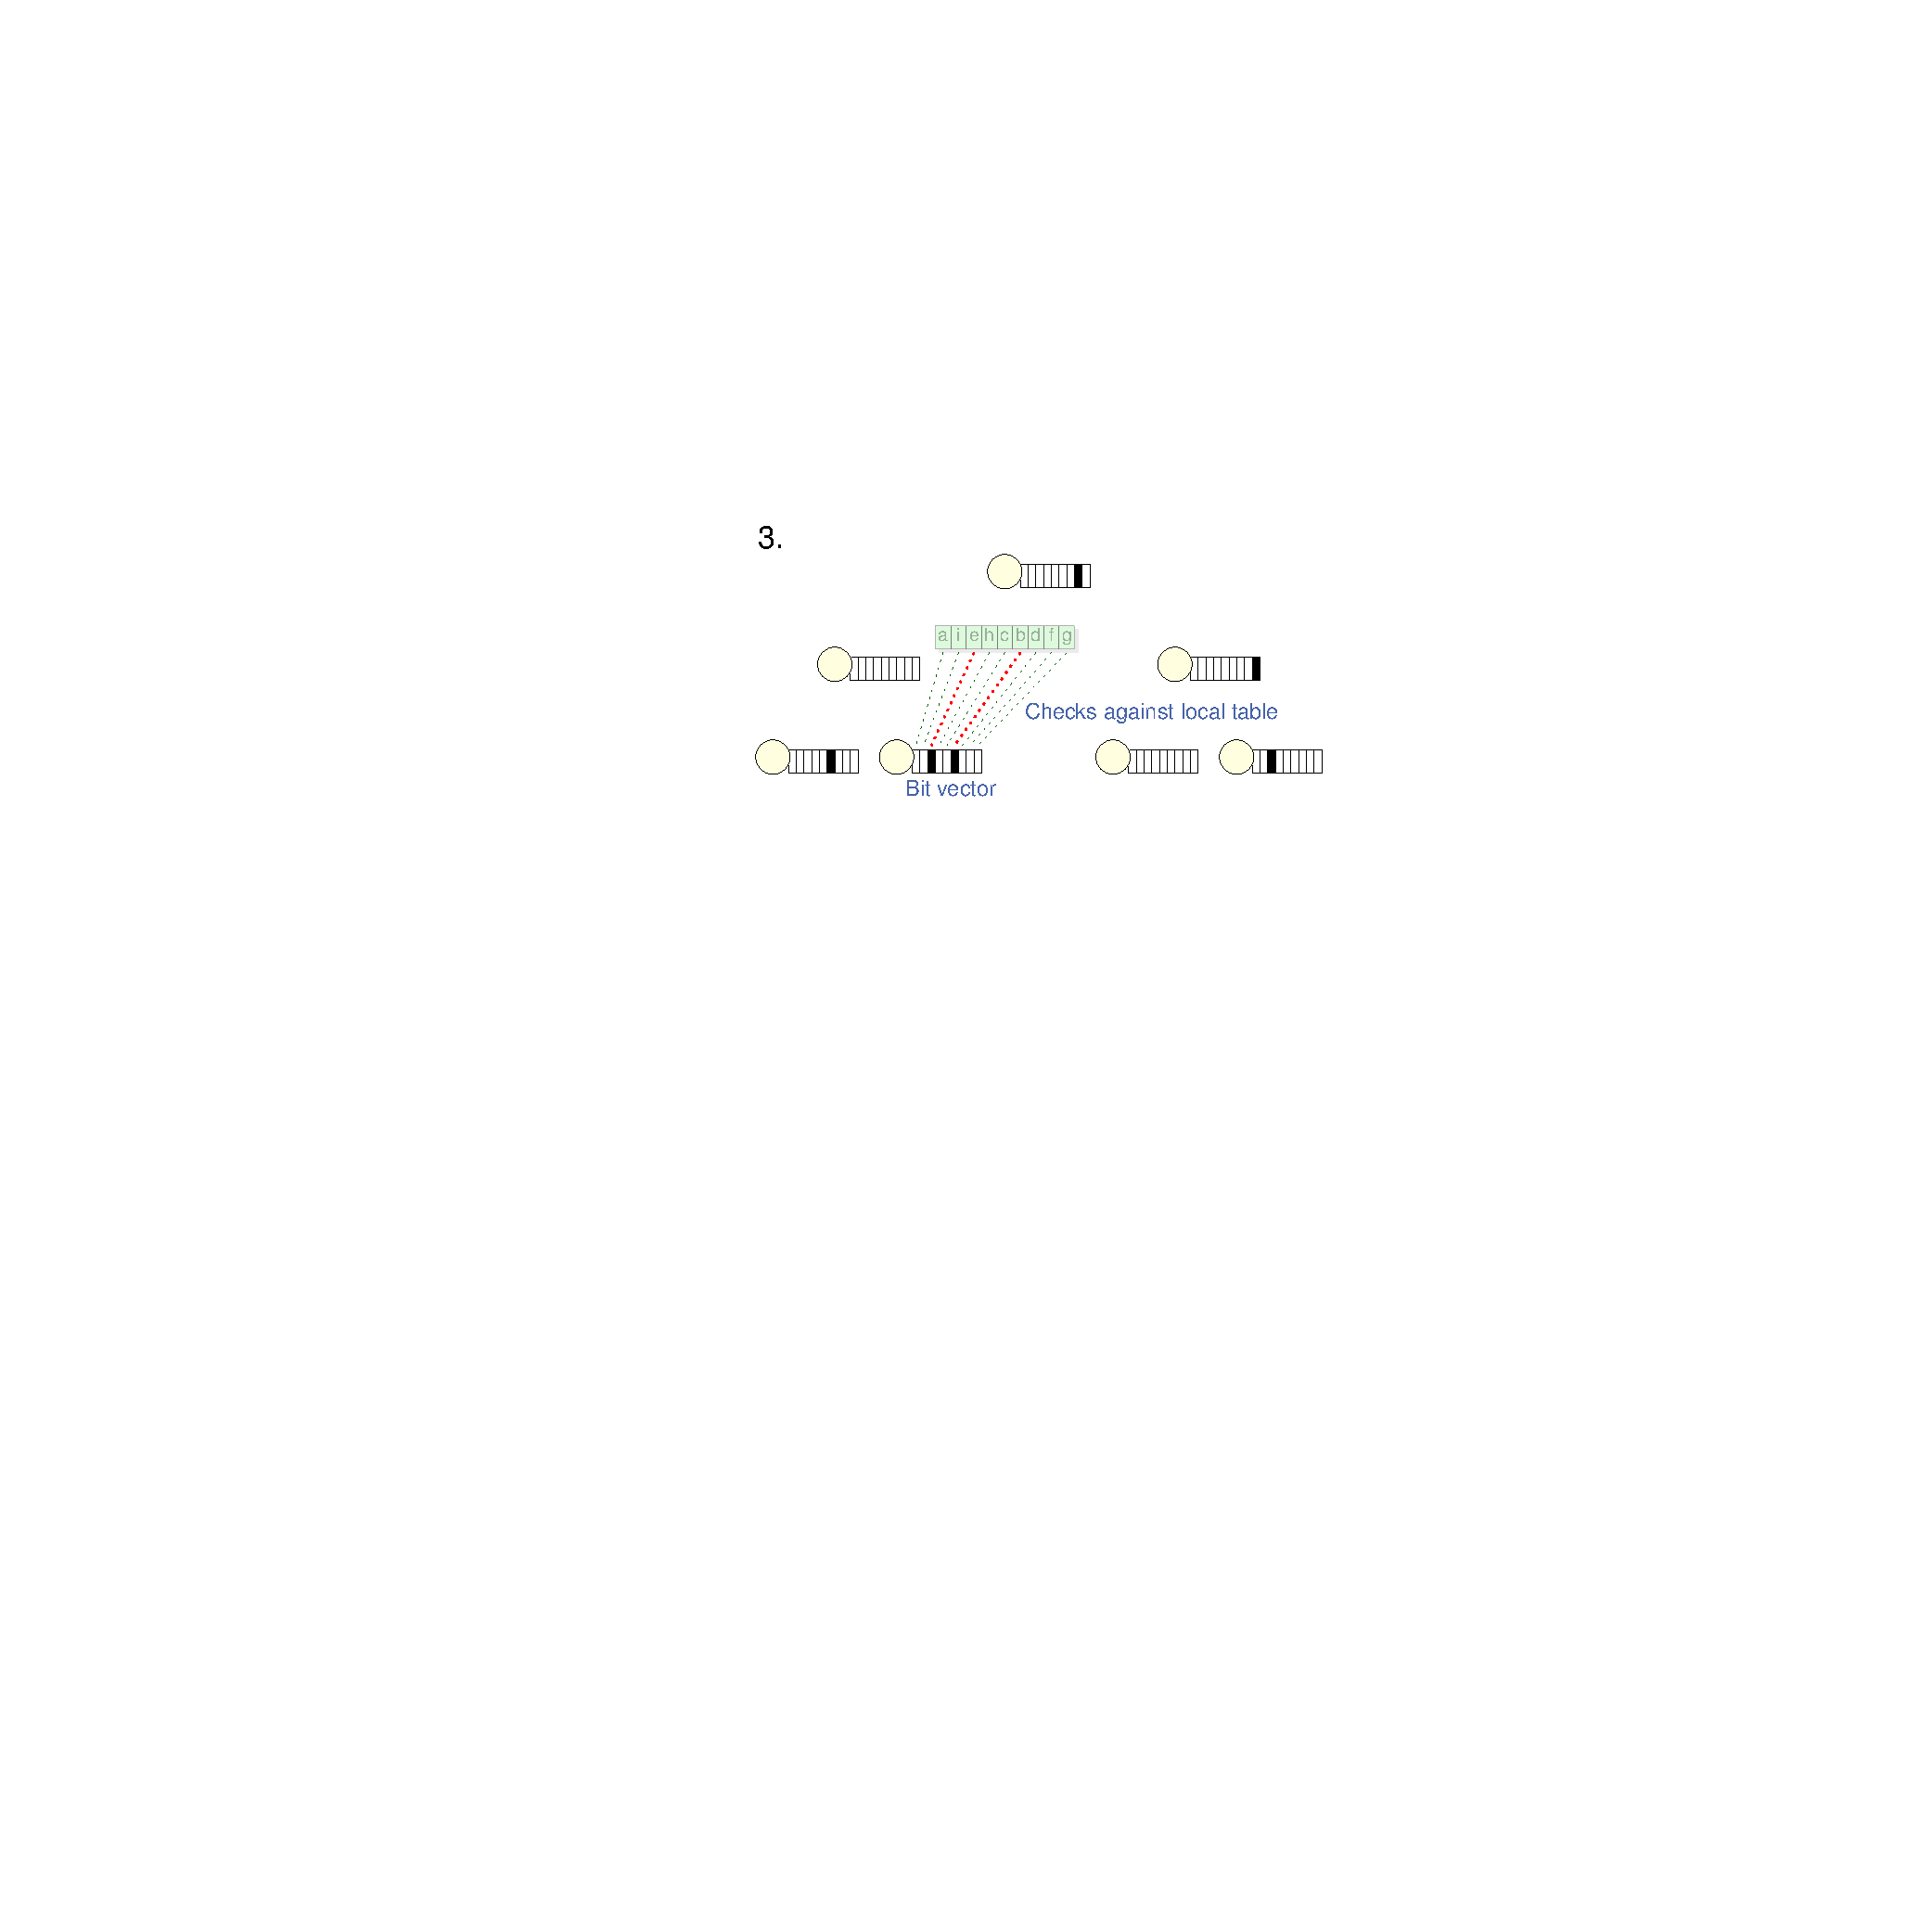
\includegraphics[width=\textwidth,page=1]{figures/l08/clause-filtering-mallob.pdf}}%
		\only<2>{\includegraphics[width=\textwidth,page=2]{figures/l08/clause-filtering-mallob.pdf}}%
		\only<3->{\includegraphics[width=\textwidth,page=3]{figures/l08/clause-filtering-mallob.pdf}}%
	\end{minipage}
\end{frame}

\begin{frame}{Enforcing a Sharing Volume~\cite{schreiber2024mallobsat}}
	
	\vspace*{-7mm}
	We want to share $L$ literals per sharing but may only get $L' < L$ successfully shared literals. \highlo{Why?}
	\begin{enumerate}
		\item Processes \highl{didn't produce, export enough clauses}
		\item \highlo{Duplicate clauses} were detected and eliminated during aggregation
		\item \highlo{Distributed filter} blocked some of the transmitted clauses
	\end{enumerate}
	
	\vspace*{2mm}
	\uncover<2->{\textbf{Fix:} \highl{Elastic compensation} for sharing volume \highlo{unused for algorithmic reasons} (\itemnum{2}\,, \itemnum{3}\ )}
	
	\vspace*{4mm}
	\begin{center}
		\only<-2>{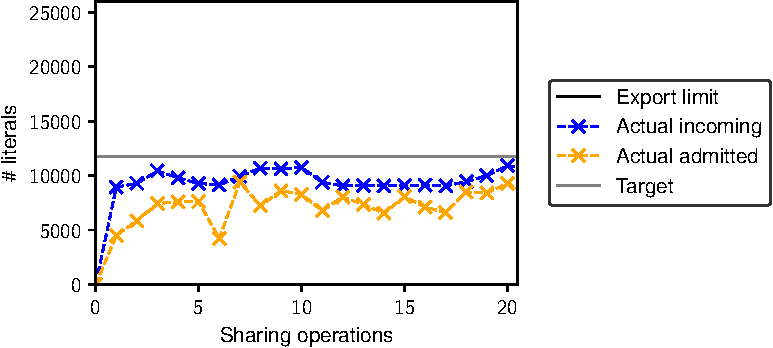
\includegraphics[width=0.6\textwidth]{figures/l08/compensation-pyplot-none.pdf}}%
		\only<3->{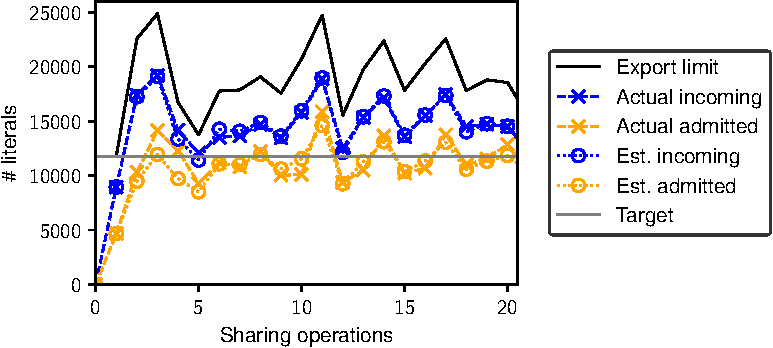
\includegraphics[width=0.6\textwidth]{figures/l08/compensation-pyplot.pdf}}%
	\end{center}
	
	%\begin{itemize}
	%	\item Track \highl{incoming}, \highl{targeted}, and \highl{actual} number of shared literals
	%	\item Compute \highl{compensation factor $\kappa$} based on \highl{elastic estimates} of the number of incoming\\
	%	and actual shared literals
	%	\item \highl{Normalize export volume per process} by $\kappa$
	%\end{itemize}
\end{frame}

\begin{frame}{Handling LBD Values}
	\begin{minipage}{0.6\textwidth}
		\vspace{0.2cm}
		\begin{itemize}
			\item Seq.\ solving: central metric for \highl{whether to keep a clause}
			\item \textbf{But:} LBD found by solver A \highlo{not necessarily meaningful}\\
			for solver B!\ \ $\rightarrow$ \highlo{not as ``global''} as clause length
			\pause
			\item Some solvers \highl{keep clauses with LBD 2 indefinitely}\\
			--- but expect \highlo{a single solver's clause volume}!\\
			$\Rightarrow$ \highlo{Growing overhead} (time, space) from low-LBD clauses
			%\pause
			%\begin{itemize}
			%	\item Use \highl{original LBD values} of imported clauses? {\small\unimp{[HordeSat]}}\\
			%	$\Rightarrow$ \highlo{Growing overhead} (time, space) from low-LBD clauses
			%	\item \highl{Reset} LBD values to \highl{maximum} at import? {\small\unimp{[TopoSAT2]}}\\
			%	$\Rightarrow$ Many clauses may be \highlo{discarded very quickly}
			%\end{itemize}
		\end{itemize}
		\vspace{0.3cm}
		\pause
		Possible approach: \highl{Increment each LBD before import}~\cite{schreiber2024mallobsat}
		\begin{itemize}
			\item Maintains \highl{LBD-based prioritization} of clauses
			\item Solver keeps \highl{more control} over its \highl{LBD-2-clauses}
			%\item ``Regional clauses are the best!''
		\end{itemize}		
		\vspace{0.3cm}
		\uncover<4->{
		\textbf{But:} Dropping LBD values alltogether performs \highl{just as well}\\
		\phantom{\textbf{But:}} in latest experiments~\cite{schreiber2025streamlining}
		}
	\end{minipage}%
	\begin{minipage}{0.4\textwidth}
		\centering
		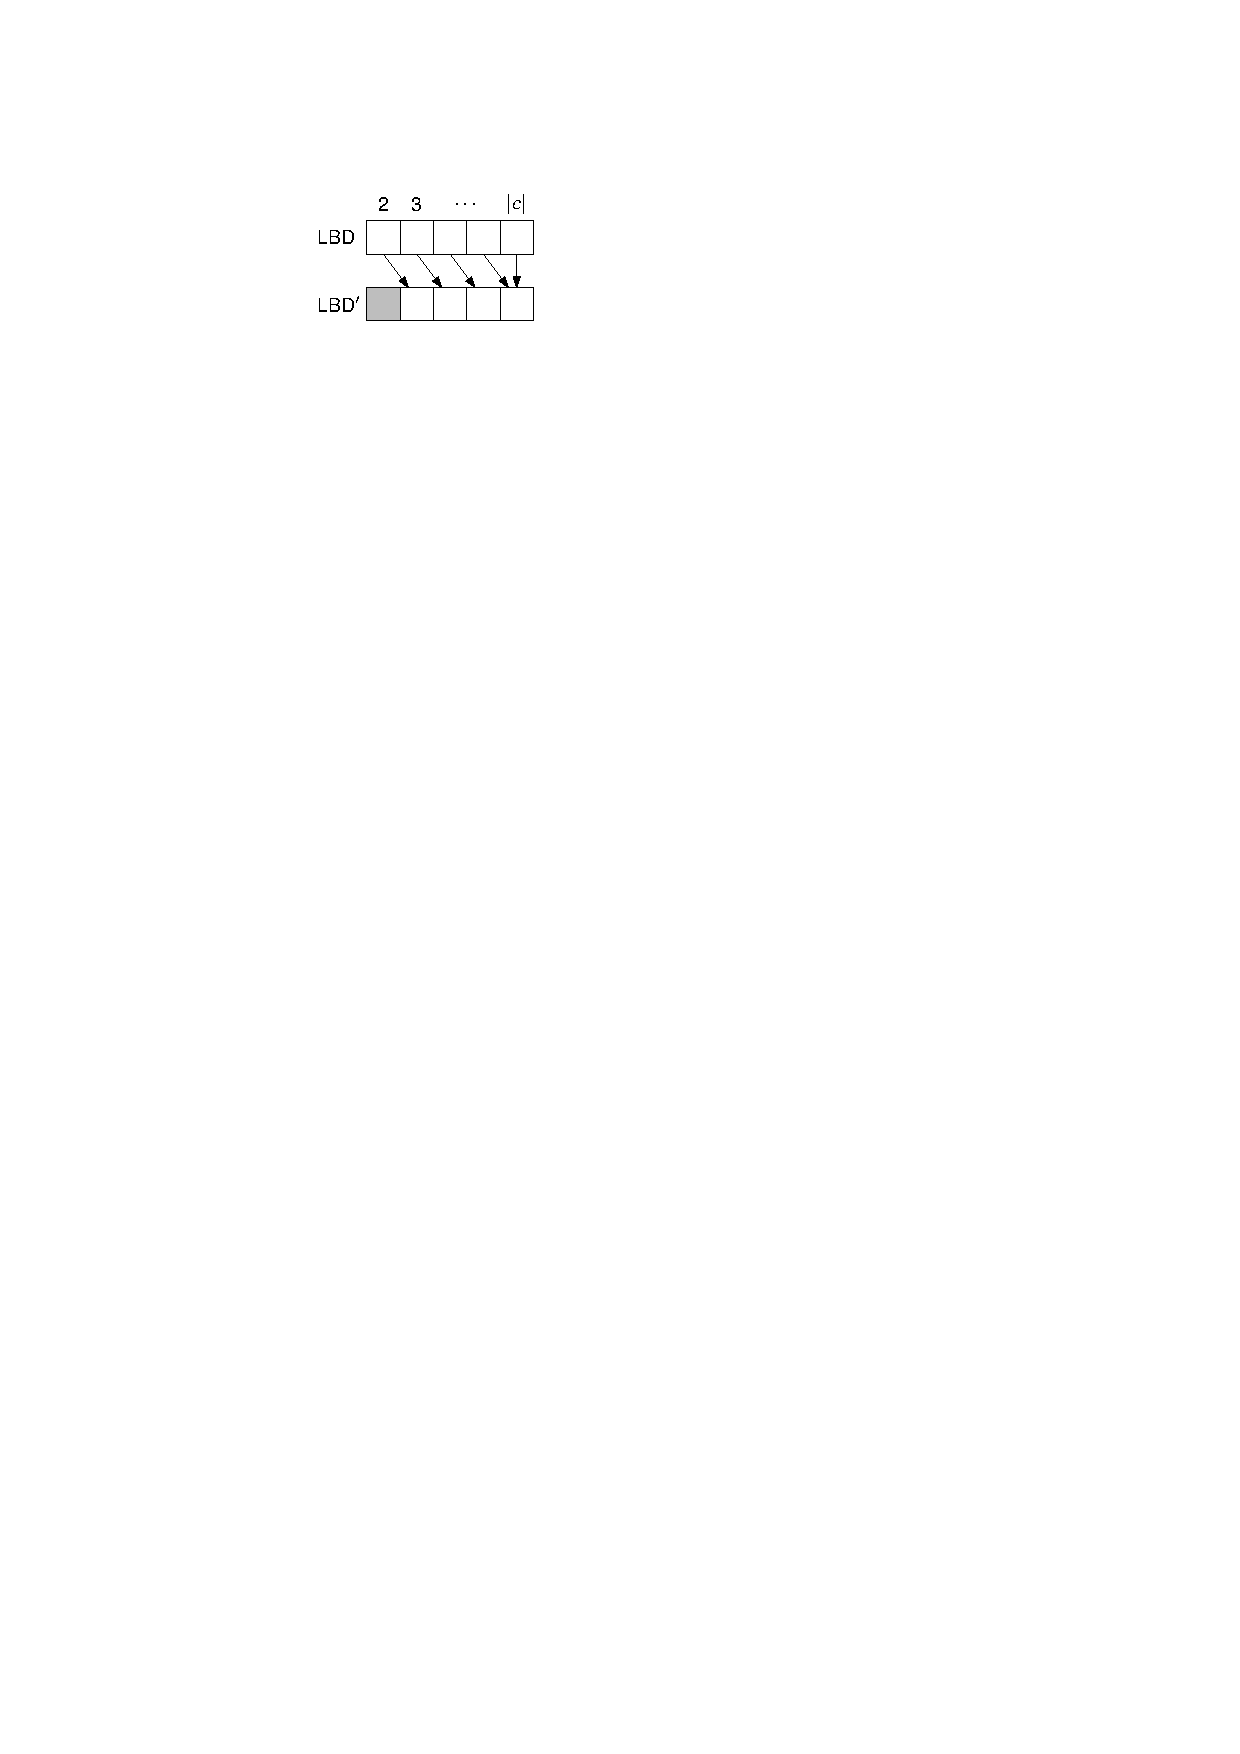
\includegraphics[width=6cm]{figures/l08/lbd-incrementing.pdf}\\[0.6cm]
		%
\includegraphics[width=0.95\textwidth]{figures/sateval-lbd-handling.pdf}
		\begin{tabular}{lrr}
			\toprule
			& Median RAM & PAR-2 \\
			\midrule
			Orig. LBD & 108.8\,GiB & 75.7 \\
			Reset LBD & 95.6\,GiB & 74.3 \\
			LBD++ & 97.3\,GiB & 72.9 \\
			\bottomrule
		\end{tabular}
		
		\vspace*{0.2cm}
		\unimp{768 cores $\times$ 349 instances $\times$ 300\,s}
	\end{minipage}%
\end{frame}

\begin{frame}{Parallel Solver Evaluation Methodology}
	Benchmark ``best'' sequential solver \unimp{(e.g., SAT Competition winner)} and parallel solver\\
	on \highl{recent competition instances}, with a fixed time limit $T$ per instance.
	\\
	\vspace*{6mm}
	\highl{Speedup} for a single instance $i$ is $s(i) := {T_{\textit{seq}}(i)} / {T_{\textit{par}}(i)}$.
	How do we compute \highl{overall speedups} over inputs $\mathcal{I}$?
	\pause
	\vspace*{2mm}
	\begin{itemize}
		\item \highlo{Arithmetic mean} $S_{\textit{arit}} = 1/|\mathcal{I}| \cdot \sum_{i \in \mathcal{I}} s(i)$~?\pause\quad\quad\highlo{No statistical meaning!}
		\pause
		\item \textbf{Median} $S_{\textit{med}}$: central item in sorted list of speedups
		\quad\quad\unimp{-- Meaningful, very conservative}
		\pause
		\item \textbf{Geometric mean} $S_{\textit{geo}} = \sqrt[|\mathcal{I}|]{\big(\prod_{i \in \mathcal{I}} s(i)\big)}$
		\quad\quad\unimp{-- Meaningful, conservative, only for running times $> 0$}
		\pause
		\item \textbf{Total} $S_{\textit{tot}} = \frac{\sum_{i \in \mathcal{I}} T_{\textit{seq}}(i)}{\sum_{i \in \mathcal{I}} T_{\textit{par}}(i)}$
		\quad\quad\unimp{-- Meaningful (``ratio of time saved''), emphasizes difficult inputs}
	\end{itemize}
	\vspace*{6mm}
	\pause
	How do we handle instances with $T_{\textit{seq}} =$ \highlo{TIMEOUT}?
	\pause
	\vspace*{2mm}
	\begin{itemize}
		\item \highl{Reduce such occurrences} by running sequential solver \highl{(much) longer} than parallel solver
		\pause
		\item ``Generously'' \highl{assume as solved} in time $T$, or apply penalty $k \cdot T$
		\quad\quad\unimp{-- makes speedups difficult to interpret}
		\pause
		\item \highl{Omit} from speedup calculation
		\quad\quad\unimp{-- clean separation of speedups from \# solved instances}
	\end{itemize}
\end{frame}

\begin{frame}{Scaling of MallobSat~\cite{schreiber2024mallobsat}}
	
	\vspace*{-5mm}
	% - geometric speedups plot of Mallob vs. Horde 
	%   + some efficiency and weak scaling measures from the text
	%\begin{center}
	\begin{minipage}{0.5\textwidth}%
		%\vspace*{-3mm}
		\hspace*{-2mm}
		\only<1>{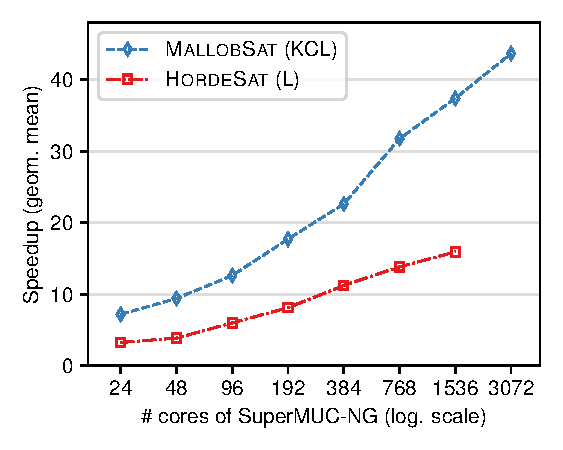
\includegraphics[width=\textwidth]{figures/l08/sateval-geomspeedups-mallob-vs-horde.pdf}}%
		\only<2->{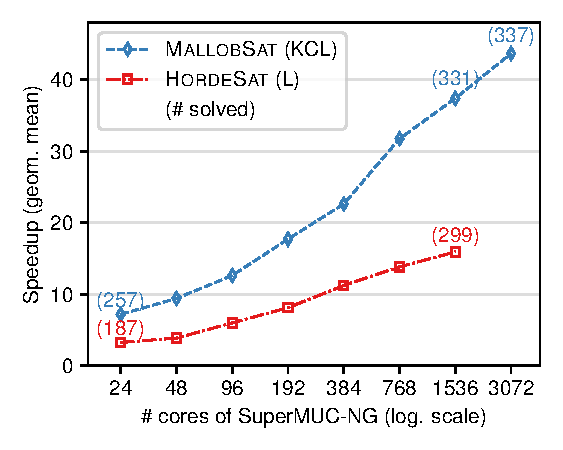
\includegraphics[width=\textwidth]{figures/l08/sateval-geomspeedups-mallob-vs-horde-toptext.pdf}}%
	\end{minipage}%
	\begin{minipage}{0.5\textwidth}%
		%\centering
		\uncover<3->{
			\vspace*{5mm}
			\begin{center}
				\textbf{Weak Scaling}
			\end{center}
			\vspace*{-3mm}
			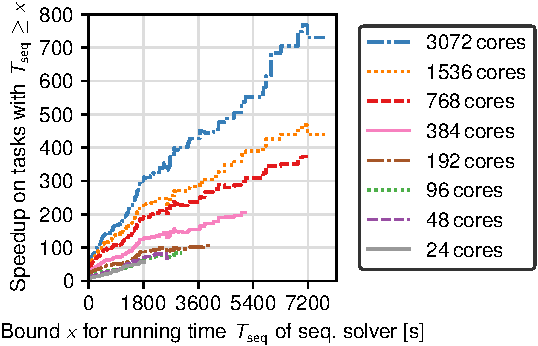
\includegraphics[width=0.95\textwidth]{figures/l08/weak-scaling-overview-crop.pdf}
		}
	\end{minipage}%
	\\[2mm]
	\unimp{
		\small
		400 problems from SAT Comp. 2021 $\cdot$
		Seq. baseline \textsc{Kissat\_MAB-HyWalk} $\cdot$
		Seq. limit 32\,h (331 solved) $\cdot$
		Par. limit 300\,s
		%\uncover<3->{Geom. Mittel der Speedups auf beiderseits gelösten Instanzen}
	}
	%\uncover<4>{\textsc{MallobSat} auf 3072 Kernen bei Problemen mit seq. Laufzeit $\geq 1$\,h:\ \ \highl{Speedup \textbf{419}} (\highl{Effizienz $\approx$ \textbf{14\%}})}
	%\end{center}
\end{frame}

\begin{frame}{Merit of Clause Sharing, SAT vs. UNSAT}
	\begin{minipage}{0.5\textwidth}
		\centering
		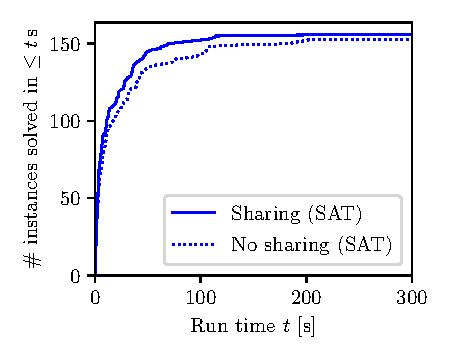
\includegraphics[width=0.9\textwidth]{figures/l08/sateval-use-of-sharing-sat.pdf}
	\end{minipage}%
	\begin{minipage}{0.5\textwidth}
		\centering
		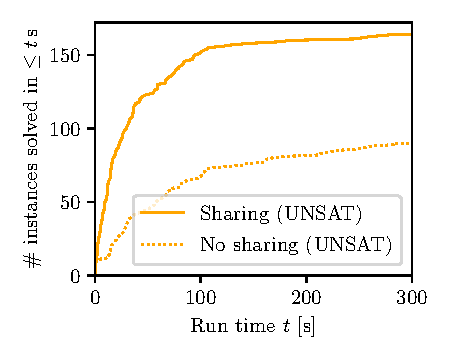
\includegraphics[width=0.9\textwidth]{figures/l08/sateval-use-of-sharing-unsat.pdf}
	\end{minipage}%
	\vspace{0.05cm}
	\centering
	\unimp{768 cores $\times$ 349 ``solvable'' instances from ISC 2022 $\times$ 300\,s, portfolio ``KCLG''}
\end{frame}

\begin{frame}{Merit of Diverse Portfolio, SAT vs. UNSAT}
	\begin{minipage}{0.5\textwidth}
		\centering
		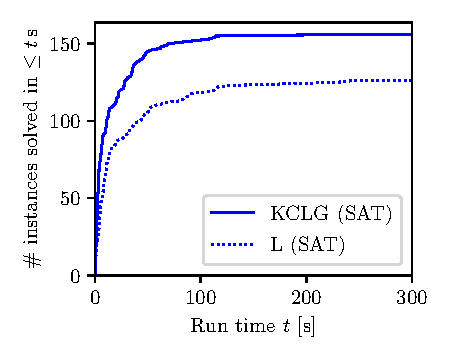
\includegraphics[width=0.9\textwidth]{figures/l08/sateval-use-of-portfolio-sat.pdf}
	\end{minipage}%
	\begin{minipage}{0.5\textwidth}
		\centering
		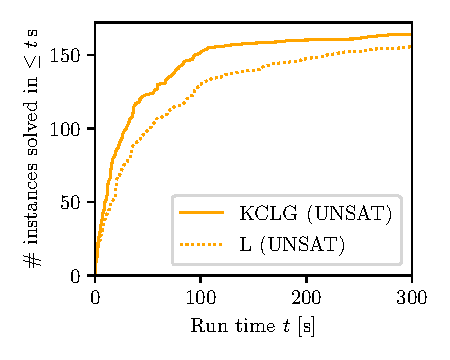
\includegraphics[width=0.9\textwidth]{figures/l08/sateval-use-of-portfolio-unsat.pdf}
	\end{minipage}%
	\vspace{0.05cm}
	\centering
	\unimp{768 cores $\times$ 349 ``solvable'' instances from ISC 2022 $\times$ 300\,s, with clause sharing}
\end{frame}

\begin{frame}{Diversification vs.\ Sharing @ 768 Cores~\cite{schreiber2024mallobsat}}
	
	\begin{minipage}{0.43\textwidth}
		\vspace*{-4mm}
		%\centering
		\only<1>{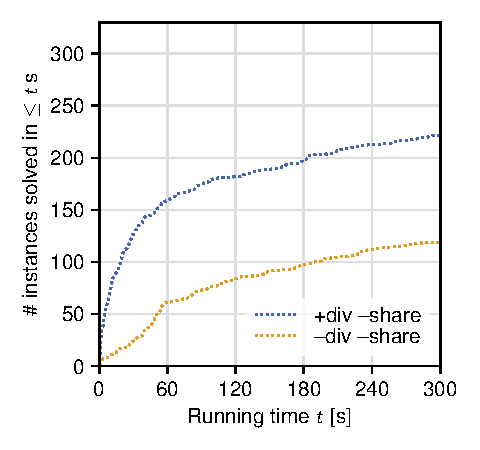
\includegraphics[width=\textwidth]{figures/l08/sateval-div-and-sharing-new-1.pdf}}%
		\only<2>{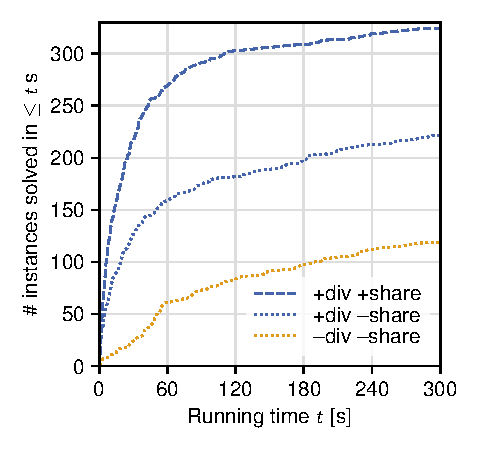
\includegraphics[width=\textwidth]{figures/l08/sateval-div-and-sharing-new-2.pdf}}%
		\only<3->{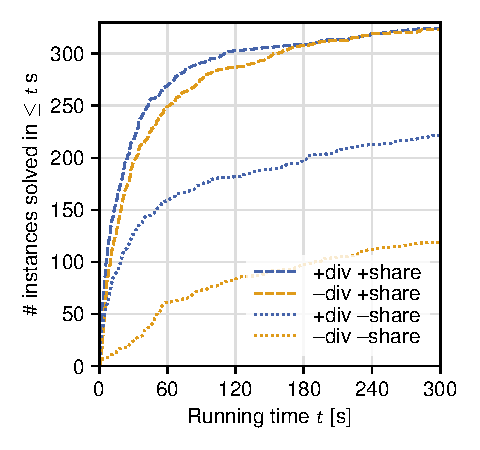
\includegraphics[width=\textwidth]{figures/l08/sateval-div-and-sharing-new-3.pdf}}%
		
		\vspace*{-1mm}
		\centering
		\unimp{\small
			349 problems from SAT Comp. 2022 $\cdot$
			CaDiCaL only}
	\end{minipage}\quad%
	\begin{minipage}{0.545\textwidth}
		\begin{itemize}
			\item \highlo{Without clause sharing}, diversification is \highl{highly effective}
			\pause
			\item With sharing:\ \ \pause 768$\times$ \highlo{the same program} \highl{performs well?!}\\[1mm]
			\pause
			$\Rightarrow$ Clause imports deviate due to parallel execution\\
			$\Rightarrow$ ``Butterfly effect'' $\rightarrow$ \highl{effective sharing}!
			%\begin{itemize}
			%	\item<3-> Threads receive shared clauses at \highl{differing points in time}
			%	\item<3-> ``\highl{Butterfly effect}'' $\Rightarrow$ deviating exploration
			%	\item<3-> Clause sharing as \highl{distributed search space pruning}
			%\end{itemize}
			\vspace*{3mm}
			%\begin{itemize}
			%	\item Sharing plus \highl{primitive diversification}\\
			%	(seeds, phases) \highl{performs competitively}
			%	\item Fully diversified portfolio without sharing \highlo{does not}
			%\end{itemize}
			%\vspace*{3mm}
			%\item<6-> \textbf{\highlo{Still a portfolio solver?}}\\
			%\uncover<7>{Rather a \textbf{\highl{clause-sharing solver}}.}
			\pause
			\item Similar findings @ 3072 cores
			\begin{itemize}
				\item Default \textsc{CaDiCaL} with \highl{primitive diversification}\\
				(seeds, phases) \highl{performs competitively}
				\item Fully diversified portfolio without clause sharing \highlo{does not}
			\end{itemize}
		\end{itemize}
		
		\pause
		\vspace*{5mm}
		$\Rightarrow$ {Portfolio of diverse configurations is \highl{dispensable}}
		\\$\Rightarrow$ {Clause sharing is \highl{essential}}
	\end{minipage}%
\end{frame}


\begin{frame}{MallobSat: A Portfolio Solver?}
	\textbf{Prevalent concept} in literature: \highlo{\textbf{Portfolio solver}} \textit{with clause sharing}\ \ /\ \ \highlo{Clause-sharing portfolio}
	\begin{itemize}
		\item ``\textit{a problem instance is independently given to a collection of solvers \highlo{competing} for a solution in parallel}''\\\hfill\unimp{-- Fichte et al., 2023}~\cite{fichte2023silent}
		\item ``\textit{each thread runs a \highlo{different SAT solver} on the same instance[, which] \highlo{in combination with} clause-sharing leads to surprisingly good performance \highlo{for small portfolio sizes}}''\hfill\unimp{-- Ozdemir et al., 2021}~\cite{ozdemir2021sat}
	\end{itemize}
	
	\pause
	\vspace*{10mm}
	\textbf{Our view}, based on empirical observations:\\[2mm]
	\highl{\textbf{\textsc{MallobSat} is a Clause-sharing solver}} \textit{with diversification}
	\begin{itemize}
		\item Clause sharing = \highl{main driver of scalability}
		\item Adding explicit diversification is \highl{beneficial but not essential}
		\item Applicability to other solvers?
	\end{itemize}
\end{frame}


\begin{frame}{Better Efficiency?}
	\begin{minipage}{0.65\textwidth}
		\vspace{0.2cm}
		\textbf{Massive parallelism for a single formula}
		\begin{itemize}
			\item \highl{Faster solving times}
			\item Can resolve problems out of reach for sequential solvers
			\item \highlo{Not that resource efficient} (on average)
		\end{itemize}
		\vspace{0.2cm}
		\pause
		\textbf{Solving many formulas in parallel}
		\begin{itemize}
			\item \highl{Embarrassingly parallel}
			\item Solving itself \highlo{less powerful}
		\end{itemize}
		\vspace{0.2cm}
		\pause
		\textbf{Best of both worlds?}~\cite{sanders2022decentralized}
		\begin{itemize}
			\item \highl{On demand scheduling} of incoming (SAT) jobs
			\item \highl{Resize jobs during their execution} as needed
			\item \highl{Few milliseconds} to schedule an incoming job,\\
			\highl{full utilization} whenever sufficient demand is present
		\end{itemize}
	\end{minipage}%
	\begin{minipage}{0.35\textwidth}
		\centering
		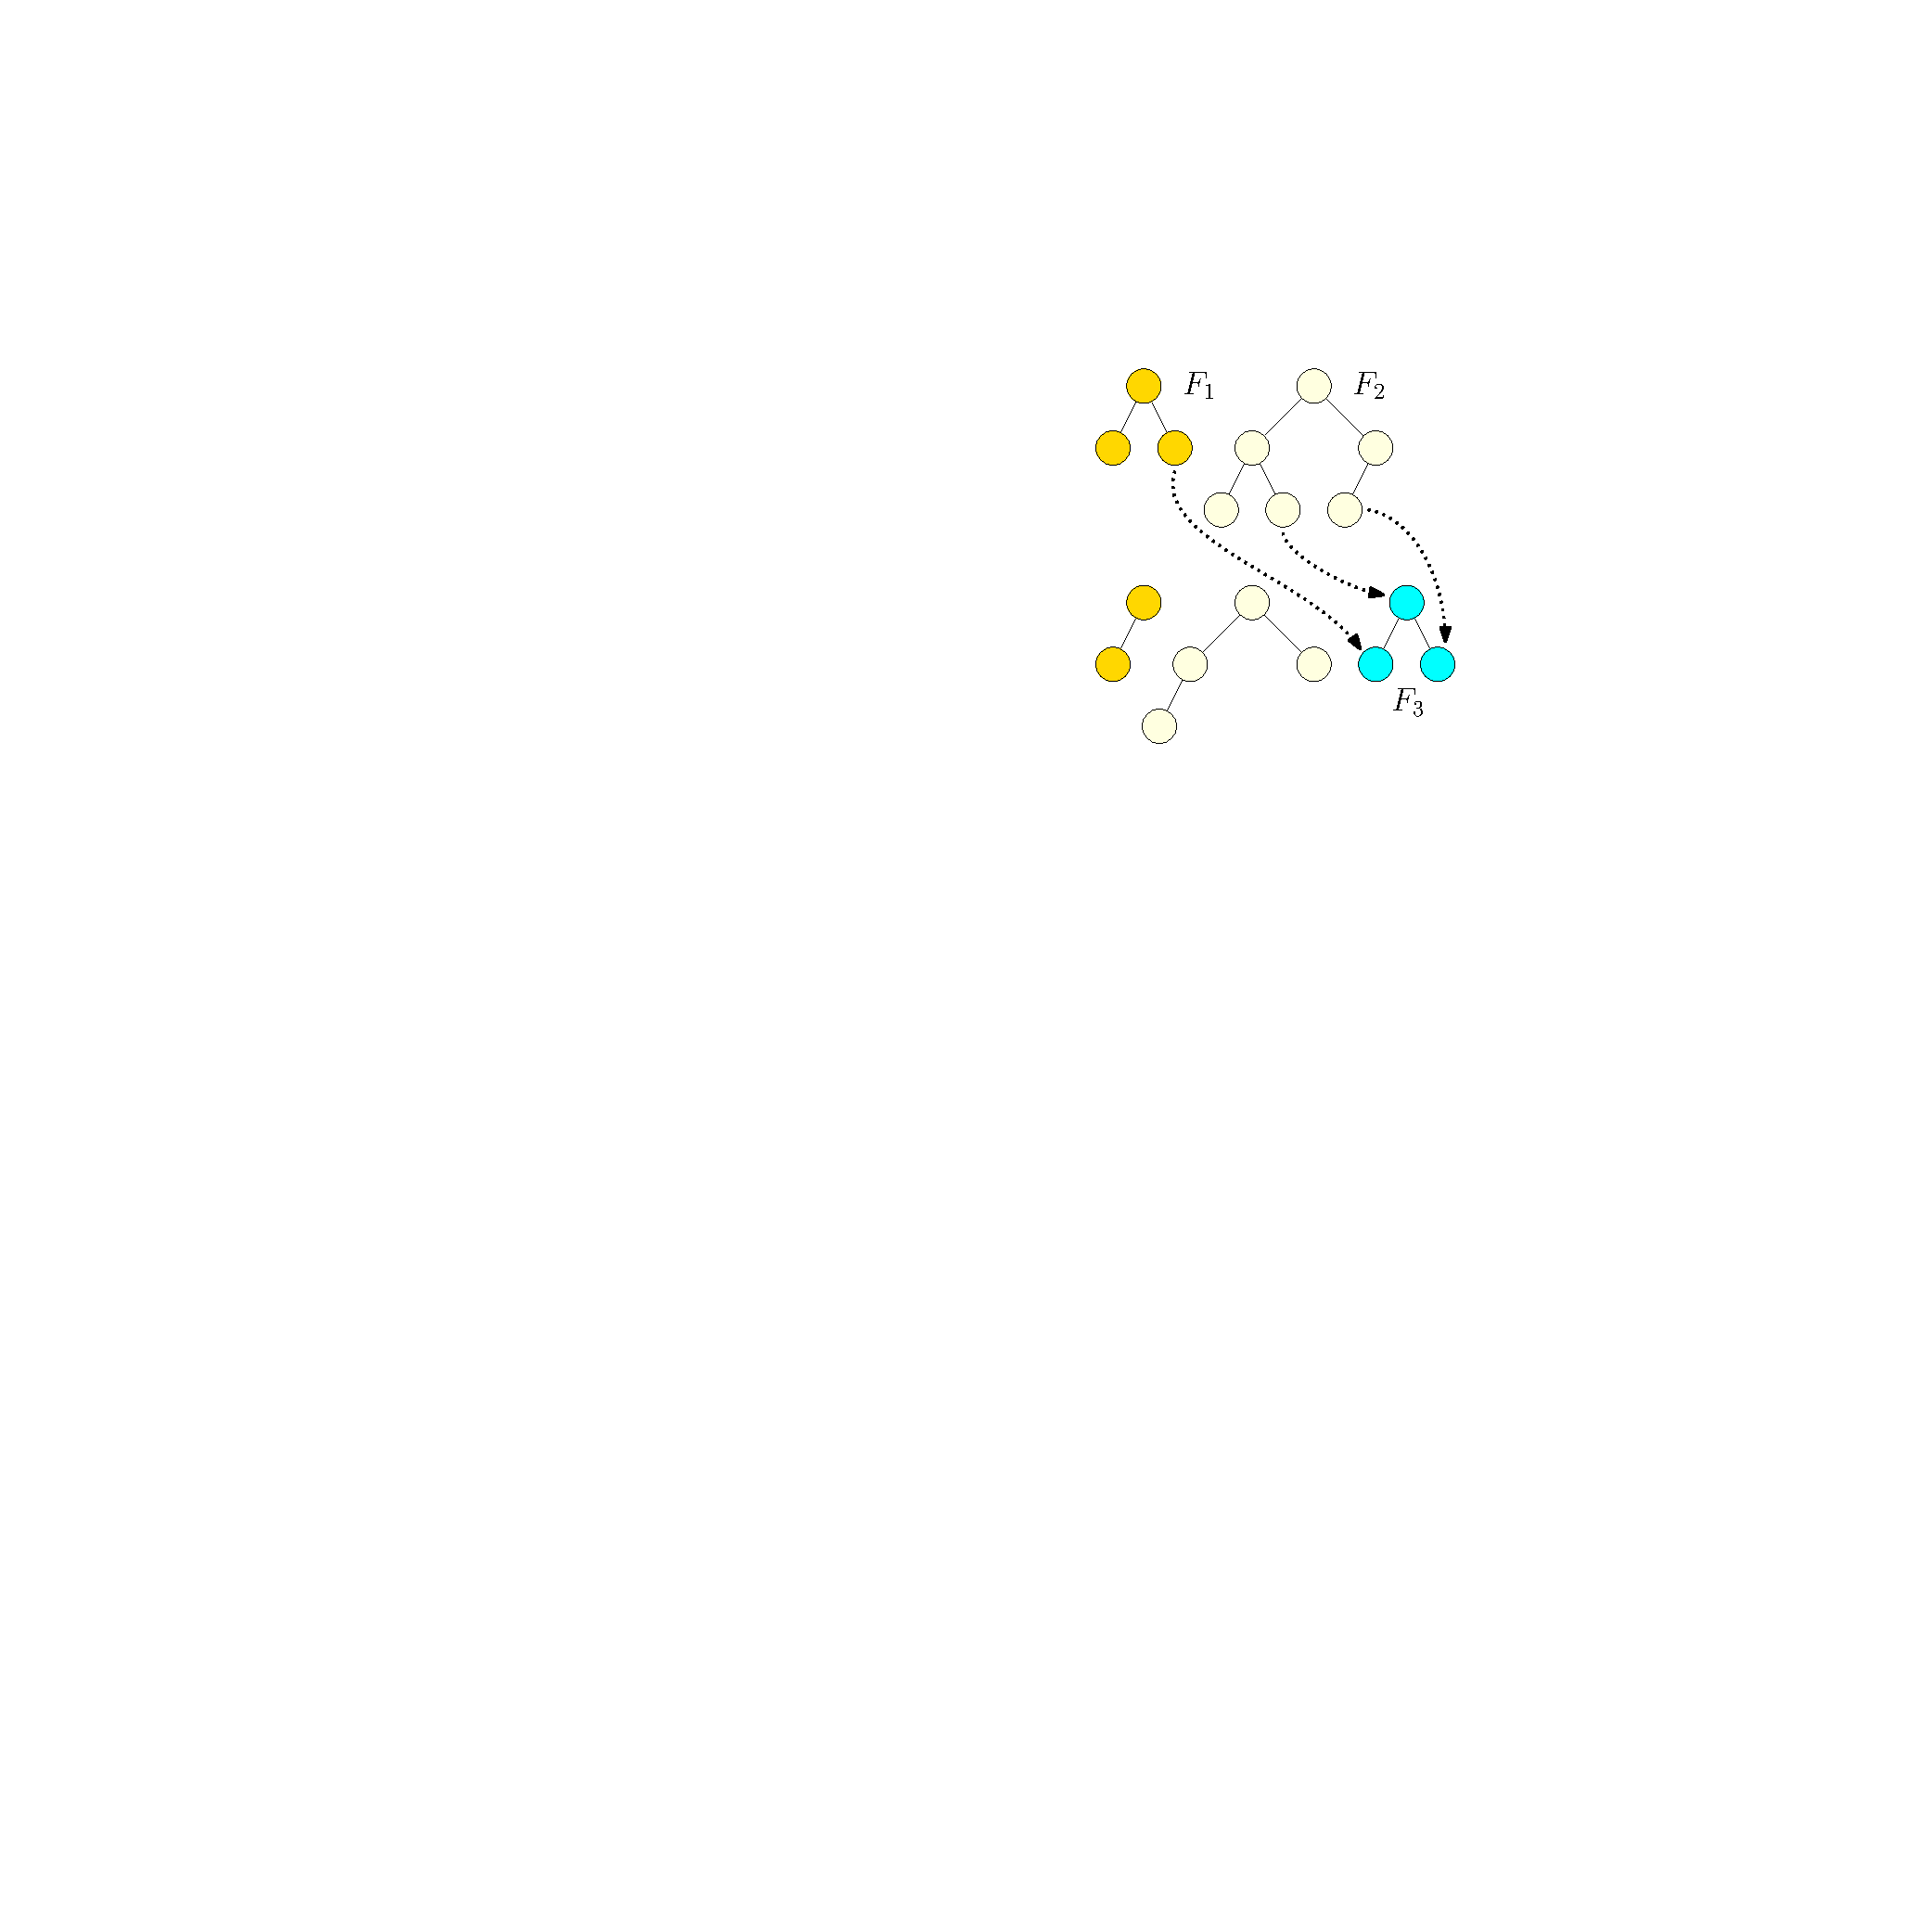
\includegraphics[width=0.85\textwidth]{figures/l08/malleability.pdf}
	\end{minipage}
\end{frame}

\begin{frame}{Scheduling Many SAT Tasks~\cite{schreiber2024mallobsat}}
	\vspace*{-1cm}
	\begin{minipage}[t]{0.55\textwidth}
		\vspace*{-6.3cm}
		\begin{exampleblock}{Problem statement}
			Given $x \in \{400,1600,6400\}$ cores and 400 SAT tasks,\\
			solve as many tasks as possible.
		\end{exampleblock}
		\vspace*{0.3cm}
		\only<2>{
			\textbf{Extreme 1:} 400 sequential solvers
			\begin{itemize}
				\item ``Embarrassingly parallel'' job processing
				%\\(\highl{inter-job parallelism})
				\item \highl{Highly efficient} (no redundant work)
				\item \highlo{Sequential solving only} $\rightarrow$ no scaling opportunity
			\end{itemize}
		}
		\only<3>{
			\unimp{\textbf{Extreme 1:} 400 sequential solvers (400$\times$\,Kissat)}\\[2mm]
			\textbf{Extreme 2:} ``Monolithic'' parallel solving
			\begin{itemize}
				\item One job at a time
				\item Generous assumption: %\highl{Optimal Offline Schedule}\\
				%--- 
				instances \highl{sorted by run time} %ascendingly
				\item Maximizes \highl{per-instance speedups}
				\item \highlo{No task parallelism}, \highlo{poor efficiency}
			\end{itemize}
		}
		\only<4>{
			\unimp{\textbf{Extreme 1:} 400 sequential solvers (400$\times$\,Kissat)}\\
			\unimp{\textbf{Extreme 2:} ``Monolithic'' parallel solving}\\[2mm]
			\textbf{Middle ground 1:} Divide cores evenly among jobs%
			\begin{itemize}
				\item \highl{Solid speedups} at small-scale parallel SAT
				%\item At the beginning, \highl{all cores are used}
				\item After $15$ min, \highlo{$>$ 50\% of cores are idling}
			\end{itemize}
		}
		\only<5->{
			\unimp{\textbf{Extreme 1:} 400 sequential solvers (400$\times$\,Kissat)}\\
			\unimp{\textbf{Extreme 2:} ``Monolithic'' parallel solving}\\
			\unimp{\textbf{Middle ground 1:} Divide cores among jobs (rigid)}\\[2mm]
			\textbf{Middle ground 2:} Divide cores \highl{dynamically} among jobs%
			\begin{itemize}
				\item Finishing jobs \highl{yield resources} to remaining jobs\\
				%--- eventually exceeding \highl{4$\times$ their initial resources}
				%\item Uses 100\% of resources 100\% of the time
				%\item @ 400 cores: \highl{Dominates} 400$\times$ Kissat!
				%\\--- shows \highl{low overhead} of scheduling
				\item<6-> \highl{Record number} of solved instances\\
				using \highl{relatively little resources}
			\end{itemize}
		}
	\end{minipage}%
	\begin{minipage}{0.45\textwidth}
		\ \ \ \ \ \ \ \ 
		\only<1-2>{\uncover<2>{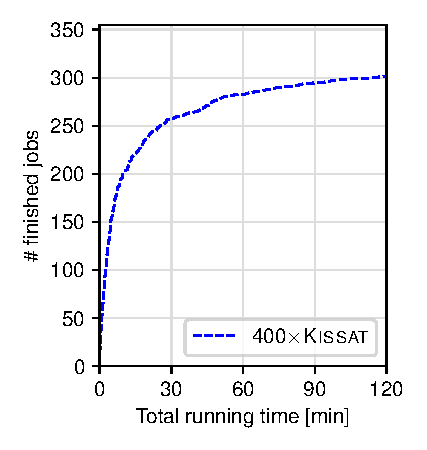
\includegraphics[width=0.93\textwidth]{figures/l08/sateval-scheduling-cdf-1.pdf}}}%
		\only<3>{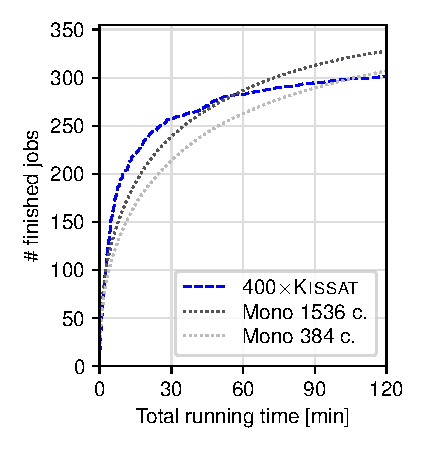
\includegraphics[width=0.93\textwidth]{figures/l08/sateval-scheduling-cdf-2.pdf}}%
		\only<4>{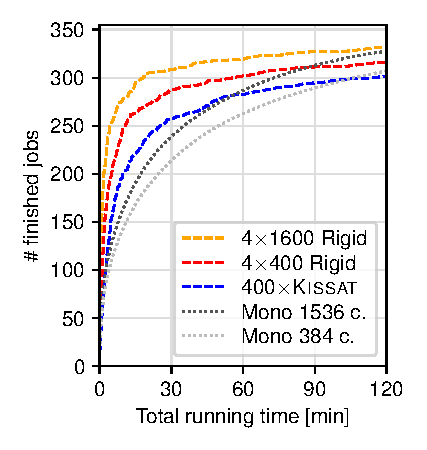
\includegraphics[width=0.93\textwidth]{figures/l08/sateval-scheduling-cdf-3.pdf}}%
		\only<5>{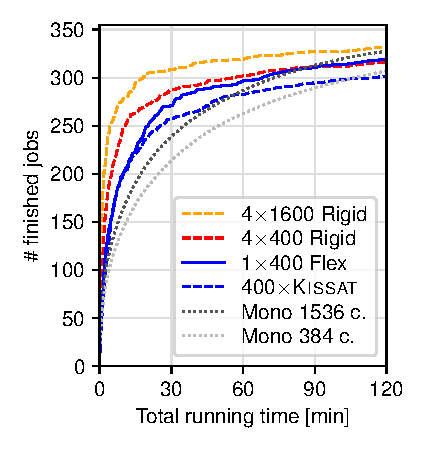
\includegraphics[width=0.93\textwidth]{figures/l08/sateval-scheduling-cdf-4.pdf}}%
		\only<6>{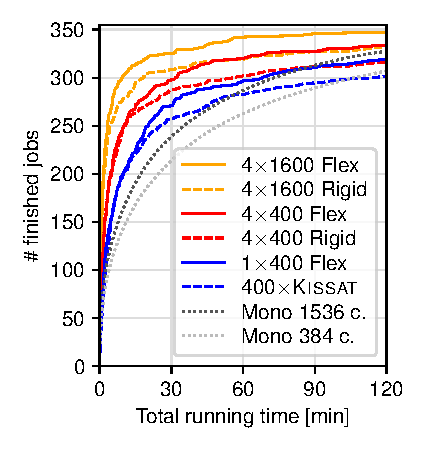
\includegraphics[width=0.93\textwidth]{figures/l08/sateval-scheduling-cdf-5.pdf}}%
	\end{minipage}
\end{frame}






\begin{frame}{Current Frontiers}
	\vspace*{-5mm}
	\begin{itemize}
		\item Streamlined \highl{clause-sharing solver} design, away from portfolios~\cite{schreiber2025streamlining}
		\\
		\vspace*{2mm}
		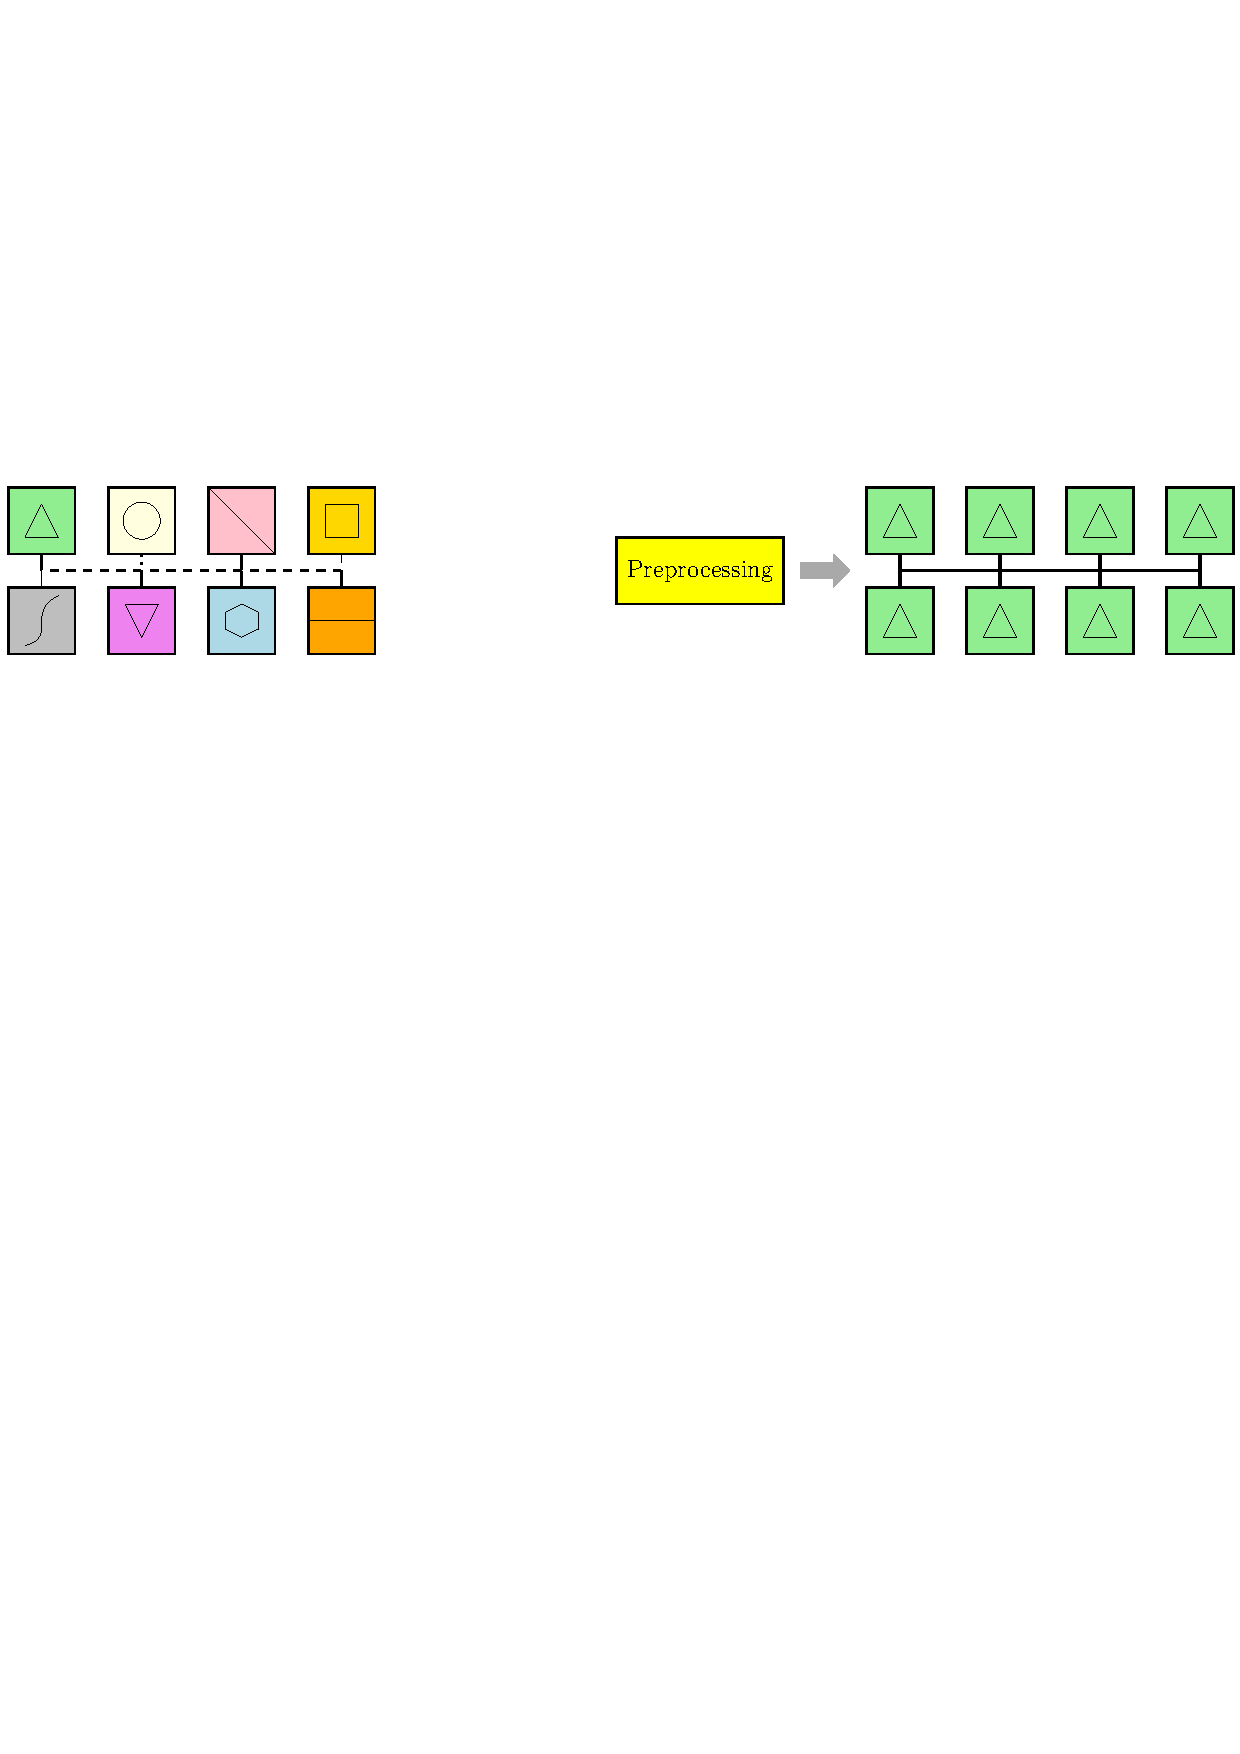
\includegraphics[width=0.9\textwidth]{figures/l08/streamlined-design.pdf}
		\\\unimp{Clause sharing portfolio with ``language barriers'' \textbf{vs.}~streamlined parallel CDCL}
		\vspace*{2mm}
		\pause
		\item Address \highlo{high main memory requirements}, especially for huge formulas (cf.~\cite{biere2022scalable})
		\vspace*{2mm}
		\item Preprocessing and Inprocessing in parallel SAT solving (cf.~\cite{osama2023certified})
		\vspace*{2mm}
		\pause
		\item Applying technology to related tools, applications
		\\-- \highl{Verification} (Bounded Model Checking, SMT Solving)
		\\-- \highl{Optimization} (MaxSAT Solving)
		\\-- Crucial piece of technology: Distributed \highl{incremental SAT solving}!~\cite{schreiber2025distributed}
		\vspace*{2mm}
		\pause
		\item \highlo{Uses of GPUs ??} (Stochastic Local Search~\cite{cen2025massively}, Inprocessing offloading~\cite{osama2023certified}, \ldots)
		\vspace*{2mm}
		\pause
		\item \highl{Proofs of unsatisfiability} (next lecture!)
	\end{itemize}
\end{frame}




\begin{frame}{Recap}
	\begin{blueblock}{Parallel SAT Solving}
		\begin{itemize}\setlength{\itemsep}{1ex}
			\iflecture{
				\item \highl{Popular parallelization approaches} for SAT (``antisocial nerds'' analogy)\\
				--- Search space splitting, Cube\&Conquer\\
				--- Pure portfolio\\
				--- Clause sharing portfolio
			}
			%\item Mallob \highl{scales up and down} --- best at large scale, very competitive at shared-memory scale!
			\item \highl{All-to-all clause sharing} can be very useful and scalable (\highl{up and down}) \highlo{if implemented well} %Schreiber \& Sanders: Scalable SAT Solving in the Cloud. SAT 2021\\
			\\
			%--- huge for unsatisfiable, nice-to-have for satisfiable problems\\
			--- \highl{diversifies solvers} effectively in and of itself
			%Also see: \url{https://youtu.be/DuM5hkSX-58}
			%\item Sanders \& Schreiber: Decentralized Online Scheduling of Malleable NP-hard Jobs. Euro-Par 2022 (in press)
			%\item Repository: \url{https://github.com/domschrei/mallob}
			\item Exploit \highl{embarrassingly parallel job processing} for interactive solving \& best efficiency
		\end{itemize}
	\end{blueblock}
	
	\begin{block}{Next Up}
		\begin{itemize}
			\item Proof pragmatics: Formats for different proof systems in the wild
			\item Bringing proof technology to parallel and distributed SAT solving
		\end{itemize}
	\end{block}
\end{frame}


\begin{frame}[allowframebreaks]{References}
	\renewcommand*{\bibfont}{\footnotesize}
	\printbibliography[heading=subbibliography]
\end{frame}

\end{document}
